%%%%%%%%%%%%%%%%%%%%%%%%%%%%%%%%%%%%%%%%%%%%%%%%%%%%%%%%%%%%
% Pedro Brandão's trial to get a template for thesis for students
% Used the upthesis from Fernando Silva (see upthesis).
% See also the packages file.
% 2014/07/07 First draft
% 2014/07/21 
%  pbrandao: added the list of listings (it should produce portuguese name if
%           babel is set to portuguese, see packages.tex). Changed usepackage of babel
%           to be before input packages.tex to allow test

%
%%%%%%%%%%%%%%%%%%%%%%%%%%%%%%%%%%%%%%%%%%%%%%%%%%%%%%%%%%%%


% makes all pages the height of the text on that page. No extra vertical space is added.
\raggedbottom 
% setting it to report will remove the blank pages before each chapter
\documentclass[11pt,a4paper,twoside]{book}


%%%%%%%%%%%%%%%%%%%%%%%%%%%%%%%%%%%%%%%%%%%%%%%%%%%%%%%%%%%%
%%%   Packages that need to be configured for the thesis
%%%%%%%%%%%%%%%%%%%%%%%%%%%%%%%%%%%%%%%%%%%%%%%%%%%%%%%%%%%%

% Language settings
% use UKenglish for UK or leave blank for US English
% it will also change the names for some of the chapters (list of tables, figures, content,
\usepackage[UKenglish]{babel}
% \usepackage[portuguese]{babel}

%%%%%%%%%%%%%%%%%%%%%%%%%%%%%%%%%%%%%%%%%%%%%%%%%%%%%%%%%%%%
%%%   Packages uses language definitions
% see file below for more packages and settings
%%%%%%%%%%%%%%%%%%%%%%%%%%%%%%%%%%%%%%%%%%%%%%%%%%%%%%%%%%%%
\usepackage{upthesis}

\usepackage{algorithm}
\usepackage{algpseudocode}

\usepackage{tikz}
\usetikzlibrary{automata,positioning}

\usepackage[
%backref={section},
%pagebackref, % for getting references to the page where the citation is (in the biblio)
pdfpagelabels=false
]{hyperref}
\hypersetup{pdftitle={Titulo da tese}, %nao suporta acentos
   pdfkeywords ={palavras chave},
   pdfsubject = {assunto},
	bookmarksnumbered=true,
   pdfauthor ={Autor}, % see other options on manual (can be page) needs empty line on bibitem
   plainpages=false, 
   pdfborder={0 0 0},
   colorlinks,%colorlinks=false,
   breaklinks=true,
	%linktocpage= false, make page number, not text, be link on TOC, LOF and LOT 
	%hyperindex=true 	% Makes the page numbers of index entries into hyperlinks. Relays on unique page anchors (pageanchor) 
% see for colors http://mirror.ctan.org/macros/latex/contrib/xcolor/xcolor.pdf
   linkcolor=	Sepia, %MidnightBlue,% BlueViolet,%Sepia, % Color for normal internal links.
   %anchorcolor=black,% Color for anchor text.
   citecolor=RedViolet,% Color for bibliographical citations in text.
   %filecolor=cyan% Color for URLs which open local files.
   %menucolor=red% Color for Acrobat menu items.
   %runcolor=filecolor% Color for run links (launch annotations).
   urlcolor=NavyBlue% Color for linked URLs.
}
%use the same style for \url as the text
% from http://en.wikibooks.org/wiki/LaTeX/Hyperlinks#Customization
\urlstyle{same}


\begin{document}

\title{Título da Tese}
\submitionplace{Tese submetida à Faculdade de Ciências da \\
  Universidade do Porto para obtenção do grau de Mestre \\ 
  em Ciência de Computadores}
\author{Nome do autor}
\department{Departamento de Ciência de Computadores \\ Faculdade de
  Ciências da Universidade do Porto}
\submitdate{Setembro 2015}

%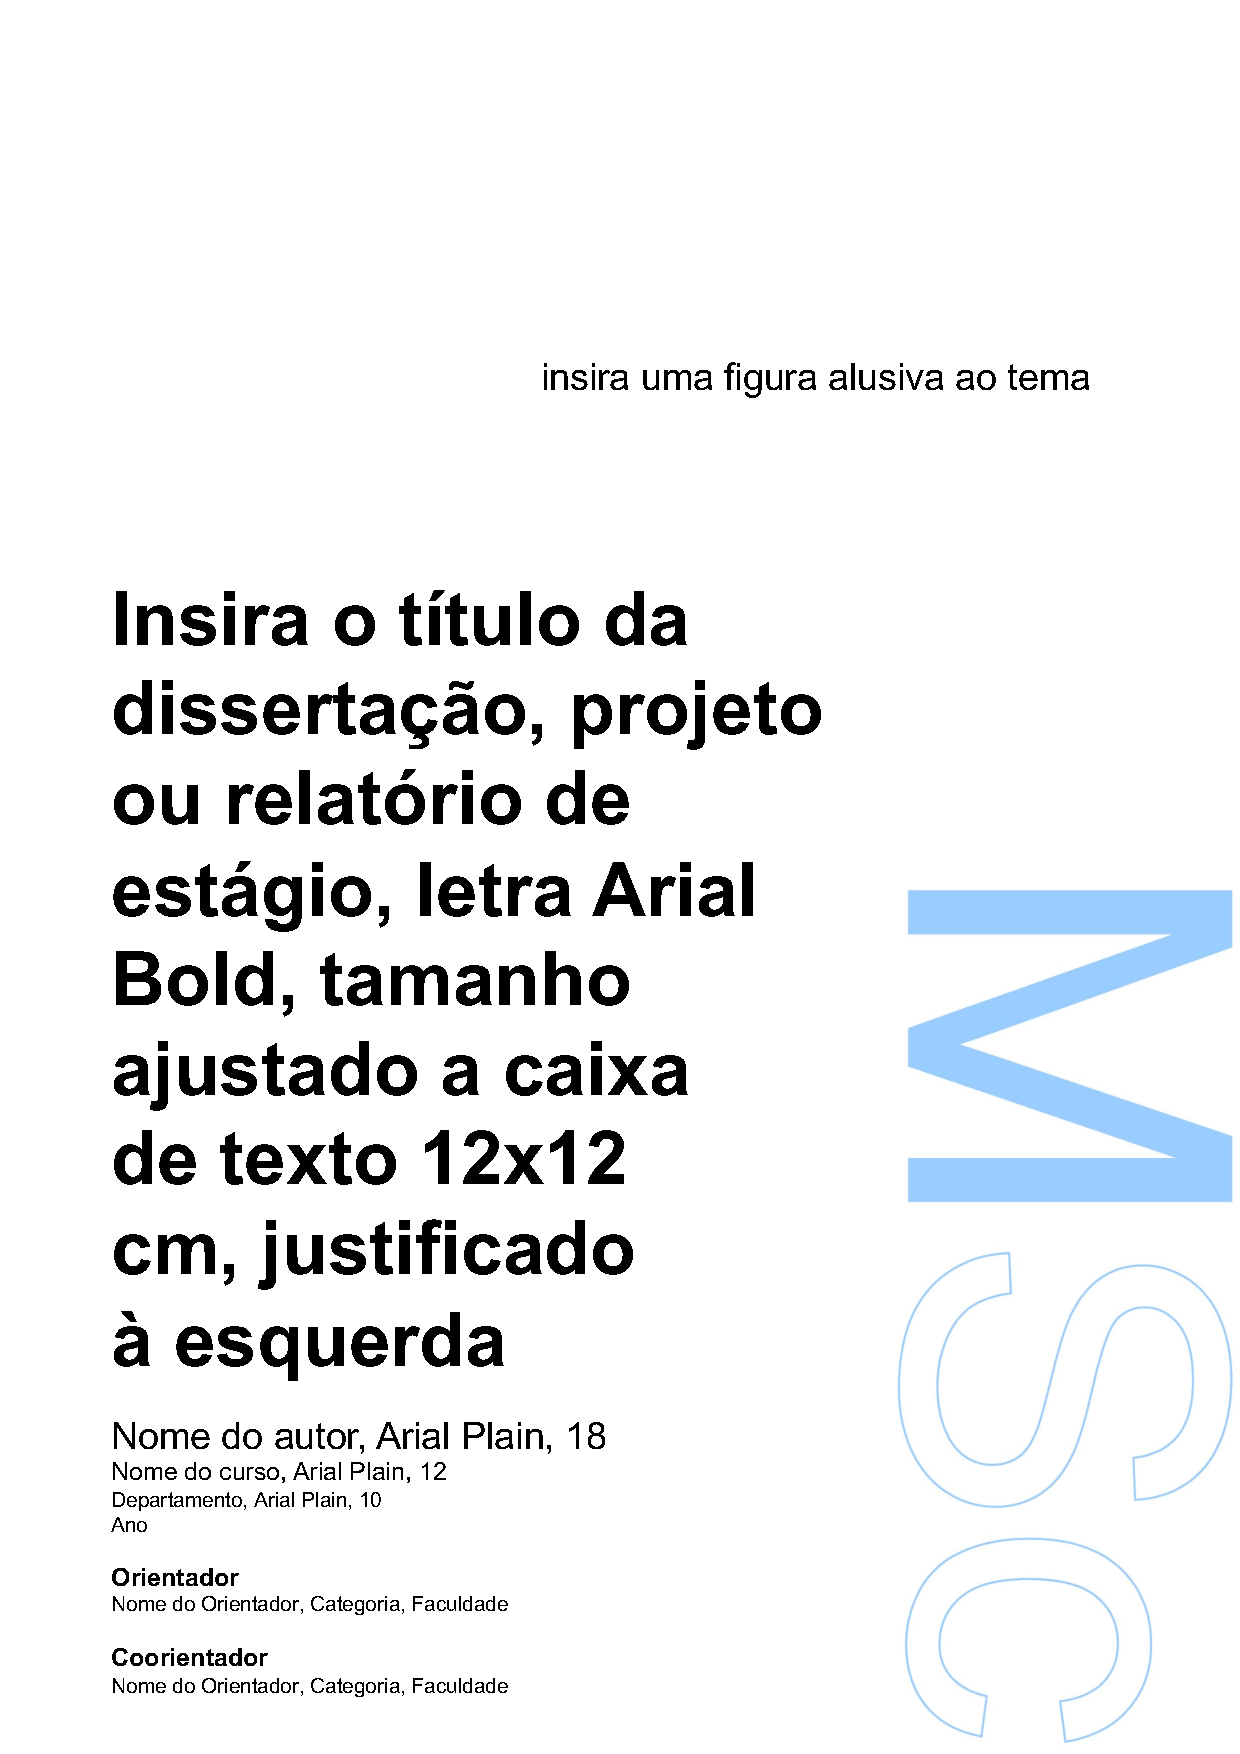
\includepdf[pages=1]{FrontPage-MSc.pdf}
%\cleardoublepage
%\includepdf[pages=2]{FrontPage-MSc.pdf}
%\cleardoublepage

\beforepreface%



% \prefacesection{Abstract}

% A long, long time ago... 

% This section should summarize the content of the dissertation, namely: explain the context of problem, describe the problem itself and address the work done to mitigate/solve the problem. Results and/or contributions should be mentioned.

% \prefacesection{Resumo}
% Há muito, muito tempo

% See the Abstract.
% Test for real
% Test

% \prefacesection{Agradecimentos}

% Obrigado a todos, obrigado \ldots

\prefacesection{Acknowledgements}
First and foremost, I want to thank professors Nelma Moreira and Rogério Reis, who have assisted me this last year. Their help, guidance, willingness and friendliness were fundamental for this work and me.
Thankfulness will never be enough to describe what I feel for my friends and family, who have helped me carry my woes and solaces along this journey. I am especially grateful to my mom and dad for taking care of me.
Lastly, I would also like to thank my work colleagues, who have been very thoughtful and patient with me along the way. 

\prefacesection{Abstract}
%Regular expressions (\emph{regex}) formalize a class of patterns definable over strings, corresponding to the family of regular languages in automata theory. They provide a declarative mechanism for specifying sets of strings, making them central both to theoretical models of computation and to practical applications such as string matching, input validation, and text parsing. Despite their utility, improperly constructed regular expressions can introduce serious security vulnerabilities. One of the most critical threats is the \ac{ReDoS} attack, in which carefully crafted inputs cause the regex engine to perform excessive and redundant processing. This results in dramatic slowdowns or even complete unresponsiveness of the system. \ac{ReDoS} poses a significant risk to web applications, APIs, and other input-facing systems, where user-controlled input is matched against vulnerable patterns.
\noindent Regular expressions (\emph{regex}) formalize a class of patterns definable over strings, corresponding to the family of regular languages in automata theory. They provide a declarative mechanism for specifying sets of strings, making them central both to theoretical models of computation and to practical applications such as string matching, input validation, and text parsing. Despite their utility, certain implementations of regular expression engines (particularly those based on backtracking) can introduce serious security vulnerabilities when combined with specific patterns. One of the most critical threats is the \ac{ReDoS} attack, in which carefully crafted inputs cause the regex engine to perform excessive and redundant processing. This results in dramatic slowdowns or even complete unresponsiveness of the system. \ac{ReDoS} poses a significant risk to web applications, APIs, and other input-facing systems, where user-controlled input is matched against vulnerable patterns.

\noindent In this work, bounded quantifiers (counting) were implemented in \textit{FAdo}. With this, we also propose a system to address \ac{ReDoS} by transforming regular expressions into a modified position automaton, a \ac{NFA} that tracks the exact start and end positions of all matches within an input string. This structure enables a matching function that computes all match positions, including overlapping ones, without relying on backtracking. By exhaustively and efficiently exploring the automaton's transitions, our approach avoids the exponential blowup typical of vulnerable engines, while preserving a somewhat full regex expressiveness.

\noindent We also review existing solutions present in state-of-the-art programming languages and libraries, such as \emph{RE\#} \cite{resharp_tool_paper} and \emph{Hyperscan} \cite{hyperscan_paper}.

\textbf{Keywords:} regular expressions, ReDoS, position automata, nondeterministic finite automata, pattern matching.

\prefacesection{Resumo}
\noindent As expressões regulares (\emph{regex}) formalizam uma classe de padrões definíveis sobre cadeias de caracteres, correspondendo à família das linguagens regulares na teoria dos autómatos. Fornecem um mecanismo declarativo para especificar conjuntos de cadeias, sendo, por isso, centrais tanto para modelos teóricos de computação como para aplicações práticas, tais como procura de padrões, validação de dados e análise de texto. Apesar da sua utilidade, certas implementações de motores de expressões regulares (particularmente aqueles baseados em \textit{backtracking}) podem introduzir vulnerabilidades de segurança graves quando utilizam padrões específicos. Uma das ameaças mais críticas é o ataque \ac{ReDoS}, onde certas entradas levam o motor de regex a realizar processamento excessivo e redundante. Isto resulta em lentidões significativas ou mesmo na completa inoperacionalidade do sistema. O \ac{ReDoS} representa um risco significativo para aplicações web, APIs e outros sistemas voltados para entrada de dados, onde a entrada controlada pelo utilizador é comparada com padrões vulneráveis.

\noindent Neste trabalho, foram implementados quantificadores limitados (contagem) no \textit{FAdo}. Com isto, propomos também um sistema para mitigar o \ac{ReDoS}, ao transformar expressões regulares num autómato de posições modificado --- um \ac{NFA} que regista exatamente as posições de início e fim de todas as ocorrências dentro de uma cadeia de entrada. Esta estrutura permite que uma função de \textit{matching} calcule todas as posições de ocorrência, incluindo as sobrepostas, sem recorrer a \textit{backtracking}. Ao explorar de forma exaustiva e eficiente as transições do autómato, a nossa abordagem evita a explosão exponencial típica de motores vulneráveis, mantendo, ao mesmo tempo, uma expressividade relativamente completa das expressões regulares.

\noindent Analisamos também soluções existentes em linguagens e bibliotecas de programação de ponta, como o \emph{RE\#} \cite{resharp_tool_paper} e o \emph{Hyperscan} \cite{hyperscan_paper}.

\textbf{Palavras-chave:} expressões regulares, ReDoS, autómatos de posições, autómatos finitos não deterministas, correspondência de padrões.

\dedicationpage{Dedico a \ldots mim}

% end of thesis preamble
\afterpreface%

%% main tex here
%% By putting the chapter names here, one can just comment the content in the chapters 
%% and produce a pdf with the correct chapter number.
%% If you want further configurability you can use subfiles package
%% https://www.ctan.org/pkg/subfiles

%\chapter{Introdução}\label{chap:intro}
% \chapter{Introduction}\label{chap:intro}

In this chapter, the problem is overviewed, the study’s importance is explained along with goals for the proposed solution. 

\section{Background}
Despite recent advances in~\cite{cloud}, .....
\chapter{Introduction}\label{chap:intro}

%https://www.usenix.org/system/files/sec22-turonova.pdf
%https://arxiv.org/abs/2407.20479
%https://www.regular-expressions.info/catastrophic.html

In this chapter, the problem is overviewed, the study's importance is explained along with goals for the proposed solution. 

\section{Background}
Regular expressions are a foundational tool in computer science, widely used in pattern matching, lexical analysis, input validation, and string processing. Their expressiveness and concise syntax make them a powerful language for describing regular languages.

% However, when implemented without care, especially in backtracking-based engines, regular expressions can become a source of serious security vulnerabilities.

A regular expression $R$ is used (along with an input $W$) in regex matching engines. The matching engines will verify if $W$ is fully matched by $R$, meaning that the entire input is a match - or they will verify if a substring of $W$ is matched by $R$. 

% Current matching engines commonly fall into one of the following categories:
% \begin{itemize}
% 	\item \textbf{Finite State Machine Regular Expression Engines}: A finite state machine (or finite \emph{automaton}) is built and evaluated using every symbol $\sigma \in W$. Used \emph{UNIX}-based systems.
% 	\item \textbf{Backtracking Regular Expression Engines}: Instead of building a finite state machine, 
% \end{itemize}

\section{Regular Expression Denial of Service}
One such vulnerability is known as \emph{Regular Expression Denial of Service} (ReDoS). ReDoS exploits the pathological worst-case behavior of certain regular expressions, causing exponential time complexity during matching. In typical backtracking matchers---such as those found in JavaScript, Java, and many scripting environments---ambiguous or nested expressions (especially involving repetition, such as \texttt{(a+)+}) can lead the engine to explore an exponential number of paths for certain crafted inputs. This behavior allows an attacker to intentionally supply inputs that force excessive computation, effectively rendering a service unavailable or degraded.

The root of the ReDoS problem lies not in regular expressions as a theoretical model but in how they are operationalized in software. While deterministic finite automata (DFAs) evaluate regular expressions in linear time, many real-world engines opt for backtracking NFAs due to their flexibility and ease of implementation. Unfortunately, these NFAs are susceptible to exponential blow-up in ambiguous or unguarded patterns.

\section{}

%\chapter{Background}\label{chap:back}
% \chapter{Background}\label{chap:back}

This chapter has the ``Instructions for preparing and writing M.Sc. Dissertations'' (Research-oriented work), 
Version 1.0, January, 7$^{th}$, 2015 from prof. Inês Dutra. It was originally written in English so it was kept as such. It was some additions from Pedro Brandão.

\section{Before Starting}
%%%%%%%%%%%%%%%%%%%%%%%%%%%%%%%%%%%%%%%%
Before starting your dissertation, you need to \textbf{define} what is the subject you are going to work
with and perform a \textbf{thorough systematic} bibliography review of the theme you chose.
What is a systematic review? It is the one where you search the web or books for the subject, and
define rules for filtering papers in two sets “included” and “excluded” and explain why some papers
go to one set or the other.
In order to start the search, you need to prepare keywords related to your subject and prepare
queries to be used in Google Scholar, Scopus, MesH etc. These search engines will return a number
of papers on the subject you are looking for.\textbf{You need to read at least the abstract and 
conclusions of every paper retrieved after your search}. Now, you filter out only the ones you
think are very closely related to your research work, and give a reason for choosing those papers.

\section{Bibliography}
%%%%%%%%%%%%%%%%%%%%%%%%%%%%%%%%%%%%%%%%
 Start organizing your bibliography file. Choose one of the standards available to start organizing
your references. Usually your department/faculty has clear rules about the standard to be used. If
you are formatting your text using \LaTeX, most references found during your bibliographic search
can be exported in BibTeX format.

\subsection{Bibliography Section}
%---------------------------------------
Your dissertation needs to have a Bibliography Section with a list of the cited works you have in
the text. In the process of writing your dissertation, make sure to properly refer the authors you are
basing your text on. For example, “Yaacoub et al.~\cite{yaacoub2012} discovered that\ldots”. In this sentence, Yaacoub is the
first author of one of the publications you list in the Bibliography Section of your dissertation and~\cite{yaacoub2012} is the link that connects this citation to the publication in the bibliographic list. If your
bibliographic entry has only one author, you cite only the author's surname. If the bibliographic
entry has two authors you cite the two authors' surnames (e.g., Clausen and Jacquet~\cite{Clausen2003}). If the
bibliographic entry has more than two authors, you can use the expression “et al.”, like in the
example shown before.

You should avoid as much as possible web site references. Only in some cases, illustration, showing trends, are they acceptable.

References should be used to back up claims made. Specially in the introduction section, sentences that stipulate something should be backed by references that assert that claim (e.g.: \emph{Android, in December 2016, was the most widely used mobile operating system~\cite{netMarketShareMobileOS}\footnote{An example where a web link to a recognized market analysis company would be valid. Note that the time which the report was seen is very relevant.})}

\section{Inserts}
%%%%%%%%%%%%%%%%%%%%%%%%%%%%%%%%%%%%%%%%
Every picture, graph, diagram, algorithm, etc. needs to have a caption and a number, and needs to
be cited and explained in the text. The mere existence of a picture, etc. does not exempt it of a description. 

\subsection{Copyrights and image usage}
%---------------------------------------
If you want to use any picture, graph, diagram, etc. in your
dissertation from one of the publications, you need to make sure that you can use it (check the copyright rules). If the copyright
rules allow you to reproduce the picture (or others) in your text, you need to insert a reference to the
source (where the picture was taken from) in the caption. If you are allowed to use a picture, but
want to slightly modify it, you need to say in the caption: Adapted from [1] (where [1] is the
number of your reference in the Bibliographic Section).


\section{Chapters/Organization}
%%%%%%%%%%%%%%%%%%%%%%%%%%%%%%%%%%%%%%%%
\begin{description}
   \item[Chapter 1: Introduction:]
This should be a summary of what comes in the next chapters. Here you explain in two to five
pages: 
\begin{inparaenum}[(1)]
   \item the context of your work highlighting and defining the problem you need to solve,
   \item what you want to do (objectives),
   \item why you want to do it (motivation),
   \item how you want to achieve your objectives (methodology), always supporting your text on the available literature,
   \item contributions (results that confirm that you achieved your objectives),
   \item organization of the chapters that come next.
\end{inparaenum}

\item[Chapter 2: Basic Concepts:]
In this chapter you need to present the foundations of your work: theoretical aspects, background
material, etc. All that is needed to understand the terminology and expressions used in the remaining
chapters.
\item[Chapter 3: Related Work:]
Here you need to discuss about other works in the literature that do something similar to what
you want to do. You need to cite and discuss the relevant papers you chose to include in your study
during your survey. Explain what others do, why it is not sufficient, and why you need to do what
you want to do. It is helpful to define some criteria to compare your work against others, and
build a table with main characteristics of other works contrasting to what you want to do. In other
words, in which aspects is your work different from others?
\item[Chapter 4: Your Work:] this chapter describes the contributions of the work done. If it is based on prior work (continuation of the project or using prior developed work), it should only describe what is the new work done. If references are needed, it should be clear what is the prior work and what is the new contribution.
\item[Chapter 5: Materials and Methods:] should have:
   \begin{itemize}
      \item Definition of Experiments (if any)
      \item Definition of Evaluation Metrics
   \end{itemize}
\item[Chapter 6: Results and Analysis]
\item[Chapter 7: Conclusions and Future work:] 
         this should restate the problem and iterate through the solution(s) analyzing the advantages and contributions. The limitations and unsolved problems should also be described.
         It should also describe the potentiality of new research/development that the work enables, the future work.
   \begin{itemize}
      \item Research Summary
      \item Main Findings
      \item Limitations
      \item Future Work
      \item Conclusion
   \end{itemize}
\end{description}
During writing, some of these chapters may collapse into just one.\textbf{Your work (chapters 4-7) should account for at least 50\% of your whole dissertation.}

\subsection{Contents of each chapter}
%---------------------------------------
You should start each chapter with a summary of its objective and contents, preferably relating to previous ones. At the end of the chapter provide a conclusion/summary of it, preferably connecting it to the next one.

%vim: set fo+=aw tw=80 spl=en_gb spell: syntax spell toplevel  :

\chapter{Preliminaries}\label{chap:prelim}
Theory builds upon theory, therefore it is essential to establish a solid foundation by understanding the basic concepts and terminology that compose the core topics of formal languages and automata theory.
In this chapter we begin by formally defining what a language is and then move on to describe the class of languages known as regular languages.
Along the way, we will also introduce various concepts such as finite automata (DFA, NFA) and regular expressions.

\section{Alphabets, Strings, and Languages}
\subsection*{Alphabets}

An \emph{alphabet} is a finite, non-empty set of symbols, typically denoted by the Greek letter $\Sigma$. That is,
\[
\Sigma = \{ a_1, a_2, \dots, a_n \}
\]

\noindent where each $a_i$ is a symbol in the alphabet.

For example, one can represent the binary alphabet as $\Sigma = \{ 0, 1 \}$, or the English alphabet as $\Sigma = \{ a, b, c, \ldots, z \}$.

\subsection*{Strings}
A \emph{string} over an alphabet $\Sigma$ is a finite sequence of symbols from $\Sigma$. Strings are typically denoted by $w$, and the \emph{length} of a string $w$ is denoted by $|w|$.

The set of all strings over the alphabet $\Sigma$ is denoted by $\Sigma^*$ and defined as:
\[
\Sigma^* = \{ w \mid w \text{ is a finite sequence of symbols from } \Sigma \}
\]

The unique string of length zero is called the \emph{empty string}, denoted by $\varepsilon$.
It is important to note that $\varepsilon \in \Sigma^*$.

For example, if $\Sigma = \{ 0, 1 \}$, then we have that:
\begin{center}
	$\Sigma^* = \{ \varepsilon, 0, 1, 00, 01, 10, 11, 000, 001, 010, 011, 100, 101, 110, 111, \ldots \}$
\end{center}

Where the empty string is, as mentioned above, denoted by $\varepsilon$ and also belongs to $\Sigma^*$.

\subsection*{Languages}

A \emph{language} over an alphabet $\Sigma$ is a set of strings over $\Sigma$.

\[
L \subseteq \Sigma^*
\]

That is, a language is any subset of $\Sigma^*$, possibly infinite, finite, or even empty. \newline
Since a language is a set of strings, the following standard set operations can be applied (assuming $A$ and $B$ are languages over the same alphabet $\Sigma$):

\begin{itemize}
	\item \emph{Intersection}: $A \cap B = \{ x \mid x \in A \text{ and } x \in B \}$
	\item \emph{Union}: $A \cup B = \{ x \mid x \in A \text{ or } x \in B \}$
	\item \emph{Difference}: $A \setminus B = \{ x \mid x \in A \text{ and } x \notin B \}$
\end{itemize}

Furthermore, we can also operate specifically over languages with the following operations (assuming $L_1$ and $L_2$ are languages over the same alphabet $\Sigma$):

\begin{itemize}
	\item \emph{Concatenation}: $L_1 \cdot L_2 = \{ xy \mid x \in L_1 \text{ and } y \in L_2 \}$
	\item \emph{Kleene Star}: $L^* = \bigcup_{n=0}^{\infty} L^n$, where $L^0 = \{\varepsilon\}$ and $L^n = L \cdot L^{n-1}$ for $n > 0$.
	\item \emph{Reversal}: $L^R = \{ x^R \mid x \in L \}$, where $x^R$ denotes the reversal of string $x$.
	\item \emph{Complement}: $\overline{L} = \Sigma^* - L$, i.e., the set of all strings over $\Sigma$ that are not in $L$.
\end{itemize}

These operations form the basis for reasoning about the expressiveness and closure properties of language classes such as regular, context-free, and context-sensitive languages. In particular, regular languages are closed under all the operations listed above, including union, intersection, concatenation, and Kleene star. This robustness makes them especially amenable to algorithmic manipulation, as seen in finite automata and regular expression engines.

\section{Finite Automata}
A \emph{finite automaton} is a model of computation used to recognize regular languages. It processes input strings symbol by symbol and determines whether the string belongs to the language defined by the automaton. There are two main types of finite automata:

\begin{itemize}
    \item \textbf{Deterministic Finite Automaton (DFA)}: An automaton where, for each state and input symbol, there is exactly one possible next state.
    \item \textbf{Non-deterministic Finite Automaton (NFA)}: An automaton that allows multiple possible transitions for a given state and input symbol, including transitions without consuming any input (called $\varepsilon$-transitions).
\end{itemize}

Formally defined, an NFA is a 5-tuple $(Q, \Sigma, \delta, Q_0, F)$ where:

\begin{itemize}
    \item $Q$ is a finite set of states,
    \item $\Sigma$ is the input alphabet,
    \item $\delta: Q \times (\Sigma \cup \{\varepsilon\}) \rightarrow 2^Q$ is the transition function,
    \item $Q_0 \subseteq Q$ is the set of initial states,
    \item $F \subseteq Q$ is the set of accepting (final) states.
\end{itemize}

A string $w \in \Sigma^*$ is accepted by the NFA if there exists a sequence of transitions (possibly including $\varepsilon$-moves) that consumes $w$ and ends in a state $q$ such that $q \in F$.

\begin{figure}[H]
	\centering
	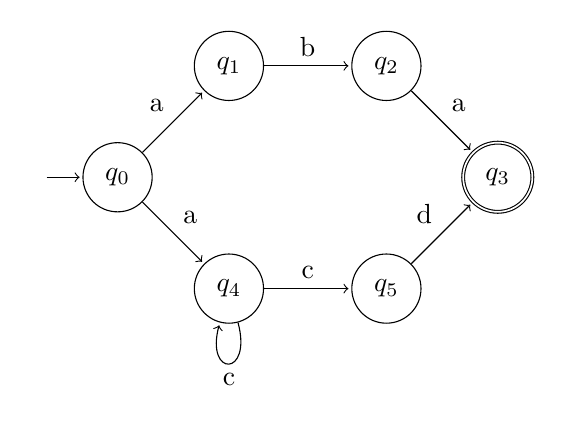
\begin{tikzpicture}[shorten >=1pt,node distance=2cm,on grid,auto,initial text=]
		\node[state, initial] (q0) {$q_0$};
		\node[state] (q1) [above right=of q0] {$q_1$};
		\node[state] (q2) [right=of q1] {$q_2$};
		
		\node[state] (q4) [below right=of q0] {$q_4$};
		\node[state] (q5) [right=of q4] {$q_5$};
		
		\node[state, accepting] (q3) [below right=of q2] {$q_3$};
		
		\path[->]
		(q0) edge node {a} (q1)
			 edge node {a} (q4)
		
		(q1) edge node {b} (q2)
		
		(q2) edge node {a} (q3)

		(q4) edge node {c} (q5)
		 	 edge[loop below] node {c} ()
		
		(q5) edge node {d} (q3);
	\end{tikzpicture}
	\caption{Example of an NFA that accepts $L = \{aba, a(c^*)d\}$}
\label{fig:nfa_example}
\end{figure}



An NFA is \emph{deterministic} (also known as DFA) if $|\delta(q,\sigma)| \leq 1$, for any $(q,\sigma) \in Q \times \Sigma$ and $|Q_0| = 1$.

\begin{figure}[H]
\centering
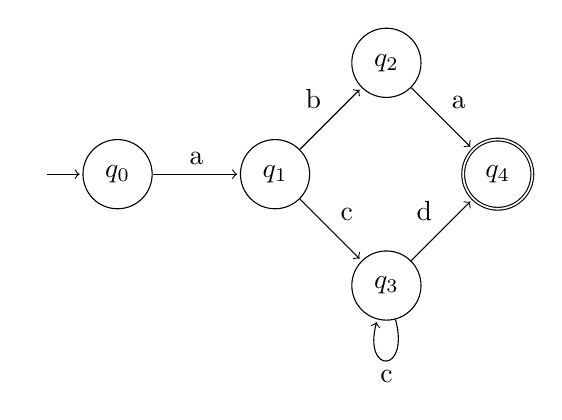
\begin{tikzpicture}[shorten >=1pt,node distance=2cm,on grid,auto,initial text=]
	\node[state, initial] (q0) {$q_0$};
	\node[state] (q14) [right=of q0] {$q_1$};
	\node[state] (q2) [above right=of q14] {$q_2$};
	\node[state] (q45) [below right=of q14] {$q_3$};
	\node[state, accepting] (q3) [above right=of q45] {$q_4$};

    \path[->]
    	(q0) edge node {a} (q14)
    	
    	(q14) edge node {b} (q2)
    		  edge node {c} (q45)
    	
    	(q2) edge node {a} (q3)
    	
    	(q45) edge[loop below] node {c} (q45)
    		  edge node {d} (q3);
  
\end{tikzpicture}
\caption{A DFA whose language is the same as the NFA from figure \ref{fig:nfa_example}} 
\end{figure}

\section{Regular Expressions}
Let $\Sigma$ be a finite alphabet. Let $L \subseteq \Sigma$. The set of \emph{regular expressions} over $\Sigma$, denoted by $\text{RegExp}(\Sigma)$, is defined inductively as follows:

\begin{itemize}
    \item $\emptyset$ is a regular expression denoting the empty language: $L(\emptyset) = \emptyset$.
    \item $\varepsilon$ is a regular expression denoting the language containing only the empty string: $L(\varepsilon) = \{ \varepsilon \}$.
    \item For each symbol $a \in \Sigma$, $a$ is a regular expression denoting the singleton language: $L(a) = \{ a \}$.
    \item If $r_1$ and $r_2$ are regular expressions, then so are:
    \begin{itemize}
        \item $(r_1 \mid r_2)$, denoting the union: $L(r_1 \mid r_2) = L(r_1) \cup L(r_2)$.
        \item $(r_1 \cdot r_2)$, denoting concatenation: $L(r_1 \cdot r_2) = L(r_1) \cdot L(r_2)$.
        \item $(r_1)^*$, denoting Kleene star: $L(r_1^*) = (L(r_1))^*$.
    \end{itemize}
\end{itemize}

For each $r \in \text{RegExp}(\Sigma)$, the function $L(r)$ yields the language defined by $r$.

Parentheses are used to disambiguate expressions and enforce precedence; by convention, Kleene star binds most tightly ($a^*$), followed by concatenation (e.g. $a \cdot b$, whose operator "$\cdot$" is omitted for convenience), and finally union ($+$).

We denote by $\alpha = \beta$ if two regular expressions $\alpha$ and $\beta$, both over $\Sigma$, represent the same language ($L(\alpha) = L(\beta)$).
Furthermore, if both expressions can be decomposed in a way that they still represent the same language, they are denoted by $\alpha \equiv \beta$.

If the language of a regular expression $\alpha$ contains the empty word, then that regular expression possesses the \textit{empty word property}.

\begin{defn}[Empty Word Property]
	The empty word property is characterized by the function $\varepsilon : \text{RegExp} \rightarrow \{ \varepsilon, \emptyset \}$ and is defined recursively as follows, given $\alpha$ and $\beta$ regular expressions defined over $\Sigma$:
	\begin{gather*}
		\varepsilon(\emptyset) = \emptyset \\
		\varepsilon(\varepsilon) = \varepsilon \\
		\varepsilon(a) = \emptyset, \: a \in \Sigma \\
		\varepsilon(\alpha + \beta) = \begin{cases}
			\emptyset & \text{if $\varepsilon(\alpha) = \varepsilon(\beta) = \emptyset$} \\
			\varepsilon & \text{if $\varepsilon(\alpha) = \varepsilon$ or $\varepsilon(\beta) = \varepsilon$}
		\end{cases} \\
		\varepsilon(\alpha \beta) = \begin{cases}
			\emptyset & \text{if $\varepsilon(\alpha) = \emptyset$ or $\varepsilon(\beta) = \emptyset$} \\
			\varepsilon & \text{if $\varepsilon(\alpha) = \varepsilon(\beta) = \varepsilon$}
		\end{cases} \\
		\varepsilon(a^*) = \varepsilon
	\end{gather*}
\end{defn}




%	\varepsilon(\alpha + \beta) = \begin{cases}
	%		
	%	\end{cases}

%	\varepsilon(\alpha + \beta) &= \emptyset \\
%	\varepsilon(\alpha + \beta), \; \text{if } \varepsilon(\alpha)\text{=}\varepsilon(\beta)\text{=}\emptyset 

%One can see if the language of a regular expression contains the empty word by utilizing the \textit{empty word property}, which is defined as the function $\varepsilon : RegExp \rightarrow \{\varepsilon, \emptyset\}$. \\
%Given $\alpha,\beta \in \text{RegExp}(\Sigma)$ and $a \in \Sigma$,



	
\subsection{Extended Regular Expressions}
\label{chap:prelim:extended_re}
In addition to the basic operations, some other operators are often used for convenience. These include:

\begin{itemize}
    \item \textbf{Kleene plus}: Given a regular expression $r$, the expression $r^+$ denotes one or more repetitions of $r$:
    \[
    L(r^+) = L(r) \cdot L(r)^*.
    \]

    \item \textbf{Fixed repetition (power)}: For a regular expression $r$ and integer $n \geq 0$, the expression $r^n$ denotes $n$ consecutive concatenations of $r$:
    \[
    L(r^0) = \{ \varepsilon \}, \quad L(r^n) = L(r) \cdot L(r^{n-1}) \text{ for } n > 0.
    \]

	 \item \textbf{Bounded repetition}: For a regular expression $r$ and integers $m, n$ with $0 \leq m \leq n-1$, the bounded repetition $r^{[m,n]}$ denotes the language containing all strings formed by concatenating between $m$ and $n-1$ copies of strings from $L(r)$:
    \[
    L(r^{[m,n]}) = \bigcup_{k=m}^{n-1} L(r^k).
    \]
\end{itemize}

These forms do not increase the expressive power of regular expressions but are useful for readability and practical applications. They can always be rewritten using the fundamental operators: union and concatenation.

\subsection{Derivatives}
\label{chap:prelim:derivatives}
% Need 1962 Janusz Brzozowski's paper for this section
The \emph{derivative of a regular expression} was first introduced in 1962 by Janusz Brzozowski. It is a powerful concept used to define the behavior of regular expressions in a more operational manner. They can be used as a means of verifying equivalence of regular expressions, for example. The derivative of a regular expression $r$ with respect to a symbol $a$ is another regular expression $d_a(r)$ that describes the set of strings that can be obtained by taking the derivative of $r$ with respect to $a$.

\begin{defn}[Derivative of a Regular Expression \cite{brzozowski_derivatives}]
	The derivative of a regular expression $r$ with respect to $\sigma \in \Sigma$ is itself a regular expression $d_\sigma(r)$ such that $\mathcal{L}(d_\sigma(r)) = \{w \ \vert \ \sigma w \in \mathcal{L}(r)\}$ and is defined as:
	\begin{align*}
		& d_\sigma(\emptyset) = \emptyset \\
		& d_\sigma(\varepsilon) = \emptyset \\
		& d_\sigma(r') = \begin{cases}
			\varepsilon & \text{if $\sigma' = \sigma$} \\
			\emptyset & \text{otherwise,}
		\end{cases} \\
		& d_\sigma(r+r') = d_\sigma(r)+d_\sigma(r') \\
		& d_\sigma(rr') = \begin{cases}
			d_\sigma(r)r' & \text{if $\varepsilon(r) = \emptyset$} \\
			d_\sigma(r)r' + d_\sigma(r') & \text{otherwise,}
		\end{cases} \\
		& d_\sigma(r^*) = d_\sigma(r)r^* \\
		& d_\sigma(r^+) = d_\sigma(r)r^*
	\end{align*}
\end{defn}


Brzozowski defined a DFA equivalent to a regular expression with the help of derivatives. With this, it is important to note that, for example, a regular expression $r = a^*$ (matches zero or more 'a' symbols) can be used to construct an equivalent DFA using Brzozowski's construction, even though $d_a(r) = a \cdot d_a(r)$ may look like it can lead to an infinite construction.

\begin{defn} [\cite{brzozowski_derivatives}]
	Two regular expressions are similar if one can be transformed to the other using only the identities:
	
	\begin{align*}
		& R + R = R, \\
		& P + Q = Q + P, \\
		& (P + Q) + R = P + (Q + R) \\
		& \varepsilon R = R \varepsilon= R \\
		& \emptyset R = R \emptyset = \emptyset
	\end{align*}
	
	Two regular expressions are dissimilar if and only if they are not similar.
\end{defn}

With this, Brzozowski proved in \cite[Theorem 5.2]{brzozowski_derivatives} that every regular expression has only a finite number of dissimilar derivatives. The big disadvantage is that, as he stated, the resulting automaton is far from minimal.

\subsection{Partial Derivatives}
The notion of \textit{partial derivative} was introduced by Antimirov \cite{pdregex_antimirov}. Opposite to Brzozowski's derivatives, \textit{partial derivatives} will lead to the construction of an NFA.

Let $\alpha \in RegExp(\Sigma)$ be a \textit{regular expression} over $\Sigma$. The set of partial derivatives of $\alpha$ with respect to a symbol $b \in \Sigma$, represented as $\partial_b(\alpha)$, is defined as follows:

\begin{align*}
	\partial_b(\emptyset) &= \emptyset		&	\partial_b(\alpha + \beta) &= \partial_b(\alpha) \cup \partial_b(\beta), \; \beta \neq \alpha \\
	\partial_b(\varepsilon) &= \emptyset	&	\partial_b(\alpha \beta) &= \partial_b(\alpha)\beta \cup \partial_b(\beta), \; \text { if } \varepsilon(\alpha) = \varepsilon \\
	\partial_b(b) &= \varepsilon & \partial_b(\alpha \beta) &= \partial_b(\alpha)\beta, \; \text { if } \varepsilon(\alpha) = \emptyset \\
	\partial_b(c) &= \emptyset, \; b \neq c \text{ and } b \in \Sigma & \partial_b(\alpha^*) &= \partial_b(\alpha)\alpha^*
\end{align*}

The set of partial derivatives by a word $w \in \Sigma^*$ 

For instance, given the regular expression $r = (ad + d^*)db$, where $\Sigma = \{a,b,d\}$, the set of partial derivatives of $r$ for the symbol $d$ is given by
\begin{align*}
	\partial_d(r) &= \partial_d((ad + d^*)db) \\
	&= \partial_d(addb + d^*db) \\
	&= \partial_d(addb) \, \cup \, \partial_d(d^*db) \\
	&= \partial_d(a)ddb \, \cup \, \partial_d(d^*)db \, \cup \, \partial_d(db) \\
	&= \emptyset ddb \, \cup \, \partial_d(d)d^*db \, \cup \, \partial_d(d)b \, \cup \, \partial_d(b) \\
	&= \emptyset \, \cup \, d^*db \, \cup \, b \, \cup \, \emptyset
\end{align*}
resulting in $\partial_d(r) = \{d^*db, b\}$.

\subsubsection{Linear Form}
\label{chap:prelim:linear_form}
It is possible to calculate the partial derivatives for every symbol $a \in \Sigma$ of a regular expression $r$ over $\Sigma$ in a single pass. To do this, Antimirov \cite{pdregex_antimirov} defined the \emph{linear form}.

A linear form $lf$ of a regular expression $\alpha$ is a finite set of symbol–continuation pairs.  
These pairs are called \textit{monomials} and they can encode all the possible one-symbol prefixes of that regular expression.

Formally, given an alphabet $\Sigma$ and the set of all regular expressions over $\Sigma$ denoted $RegExp$, a monomial is an element of $\Sigma \times RegExp$.
We denote the set of all monomials for a given alphabet $\Sigma$ by $M_\Sigma$.
  
A \emph{linear form} is then a finite set of monomials:
\[
lf(\alpha) \subseteq {2}^{M_\Sigma}.
\]

For instance, a linear form $l = \{(a_1,\alpha_1), \ldots, (a_n,\alpha_n)\}$ corresponds to the regular expression
\[
\kappa_l \;=\; a_1\cdot\alpha_1 \;+\; \cdots \;+\; a_n\cdot\alpha_n.
\]

The function $lf : RegExp \to {2}^{M_\Sigma}$ is defined recursively as follows, where $\alpha,\beta \in RegExp$:
\begin{align*}
	lf(\emptyset) &= \emptyset \\
	lf(\varepsilon) &= \emptyset \\
	lf(a) &= \{(a,\varepsilon)\}, \quad a\in \Sigma \\[4pt]
	lf(\alpha+\beta) &= lf(\alpha) \cup lf(\beta) \\
	lf(\alpha\cdot\beta) &= (lf(\alpha)\cdot \beta) \;\cup\; \begin{cases}
		lf(\beta) & \text{if } \varepsilon \in L(\alpha) \\
		\emptyset & \text{otherwise}
	\end{cases} \\
	lf(\alpha^\ast) &= lf(\alpha)\cdot \alpha^\ast
\end{align*}



%& 
%
% &  \\
%\partial_b(\alpha + \beta) = \partial_b(\alpha) \cup \partial_b(\beta), where \beta \neq \alpha

\section{From Regular Expressions to Automata}
While regular expressions provide a declarative way to specify patterns in strings, finite automata offer an operational model for recognizing such patterns.
% The equivalence between regular expressions and finite automata is not merely theoretical---it is constructive. Algorithms exist to convert any regular expression into an equivalent NFA, typically using Thompson's construction. This NFA can then be transformed into a DFA using the powerset construction, and further minimized for efficiency.

% Thompson's construction creates an NFA by recursively building automata for each component of the regular expression:
% \begin{itemize}
%     \item For a literal character, it creates a simple automaton with a single transition.
%     \item For union $R_1 \mid R_2$, it constructs a new start and accept state with $\varepsilon$-transitions to and from the sub-automata.
%     \item For concatenation $R_1 R_2$, it connects the accept state of the first to the start state of the second.
%     \item For repetition $R^*$, it creates cycles with $\varepsilon$-transitions to allow zero or more iterations.
% \end{itemize}

% The resulting NFA may be nondeterministic but is guaranteed to accept the same language as the original regular expression. Once converted into a DFA, the automaton can efficiently recognize the pattern with linear time complexity in the size of the input.

\subsection{Thompson's Algorithm}

In 1968, Thompson provided a method capable of transforming a regular expression into an equivalent nondeterministic finite automaton with $\varepsilon$-transitions (an $\varepsilon$-NFA) \cite{thompson_re2nfa}. The main idea was to associate each regular-expression operator with a small automaton fragment, and then combine these fragments recursively until the entire expression is represented.

Each basic symbol $a \in \Sigma$ is represented by two states with a transition labeled $a$ between them. The empty string $\varepsilon$ is represented by two states connected by a single $\varepsilon$-transition.

More complex expressions are built by combining smaller fragments:
\begin{itemize}
	\item Concatenation ($\alpha\beta$) is obtained by connecting the accept state of $\alpha$ to the start state of $\beta$ with an $\varepsilon$-transition.
	\item Union ($\alpha \mid \beta$) is built by adding a new start state with $\varepsilon$-transitions to the start states of $\alpha$ and $\beta$, and a new accept state with $\varepsilon$-transitions from the accept states of $\alpha$ and $\beta$.
	\item Kleene star ($\alpha^\ast$) is represented by adding a new start and accept state. The new start connects by $\varepsilon$ both to the new accept (for the empty repetition) and to the start of $\alpha$ (for one or more repetitions). The accept state of $\alpha$ connects by $\varepsilon$ back to its own start and to the new accept.
\end{itemize}

Thompson described this as a compiler-like process: the expression is first parsed into a convenient form (such as reverse Polish notation), and then a stack-based procedure builds the automaton fragment by fragment.

%\begin{algorithm}[H]
%	\caption{Thompson’s Construction}
%	\label{alg:thompson}
%	\begin{algorithmic}[1]
%		\Require $\alpha \in RegExp$
%		\Ensure $\varepsilon$-NFA $N$ such that $L(N) = L(\alpha)$
%		\Function{nfaThompson}{$r$}
%		\If{$r = \varepsilon$}
%		\State return new fragment with two states and one $\varepsilon$-transition
%		\ElsIf{$r = a \in \Sigma$}
%		\State return new fragment with two states and one $a$-transition
%		\ElsIf{$r \equiv r_1 r_2$} \Comment{Concatenation}
%		\State $N_1 \gets$ \Call{nfaThompson}{$r_1$}
%		\State $N_2 \gets$ \Call{nfaThompson}{$r_2$}
%		\State connect accept state of $N_1$ to start state of $N_2$ with $\varepsilon$
%		\State return combined fragment
%		\ElsIf{$r \equiv r_1 + r_2$} \Comment{Union}
%		\State $N_1 \gets$ \Call{nfaThompson}{$r_1$}
%		\State $N_2 \gets$ \Call{nfaThompson}{$r_2$}
%		\State create new start and new accept states
%		\State connect new start to starts of $N_1$ and $N_2$ with $\varepsilon$
%		\State connect accepts of $N_1$ and $N_2$ to new accept with $\varepsilon$
%		\State return combined fragment
%		\ElsIf{$r \equiv r_1^*$} \Comment{Kleene star}
%		\State $N_1 \gets$ \Call{nfaThompson}{$r_1$}
%		\State create new start and new accept states
%		\State connect new start to new accept with $\varepsilon$
%		\State connect new start to start of $N_1$ with $\varepsilon$
%		\State connect accept of $N_1$ back to its start and to new accept with $\varepsilon$
%		\State return combined fragment
%		\EndIf
%		\EndFunction
%	\end{algorithmic}
%\end{algorithm}

In the end, a single fragment represents the entire regular expression. The resulting automaton can be simulated efficiently by maintaining two lists of active states: the current list and the next list. For each input symbol, all $\varepsilon$-reachable states are added to the current list, transitions on the current symbol are followed, and the next list becomes the current list for the following step. A string is accepted if the accept state becomes active at the end of the input. An example of an automaton constructed using Thompson's method is shown in \ref{fig:nfa_thompson_example}.

\begin{figure}[H]
	\centering
	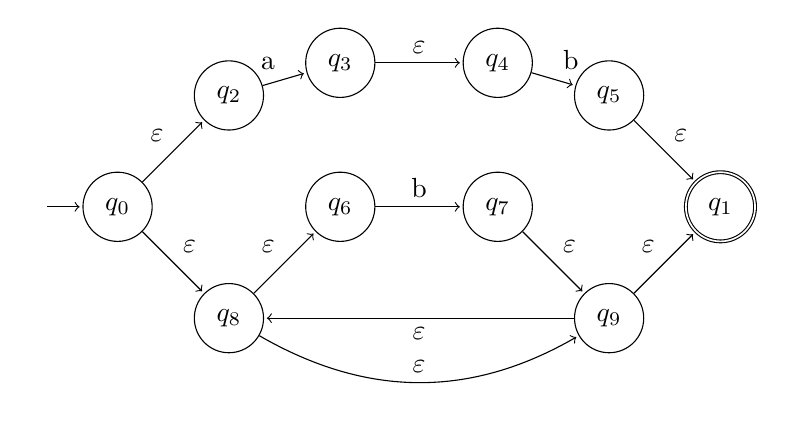
\begin{tikzpicture}[shorten >=1pt,node distance=2cm,on grid, auto,initial text=]
		\node[state,initial]	(q_0)												{$q_0$};
		
		\node[state]			(q_2)	[above right=of q_0]						{$q_2$};
		\node[state]			(q_3)	[above right=of q_2, yshift=-1cm]						{$q_3$};
		\node[state]			(q_4)	[right=of q_3]								{$q_4$};
		\node[state]			(q_5)	[below right=of q_4, yshift=1cm]						{$q_5$};
		\node[state]			(q_8)	[below right=of q_0]						{$q_8$};
		\node[state]			(q_6)	[above right=of q_8]						{$q_6$};
		\node[state]			(q_7)	[right=of q_6]								{$q_7$};
		\node[state]			(q_9)	[below right=of q_7]						{$q_9$};
		
		\node[state,accepting]	(q_1)	[above right=of q_9,below right=of q_5]		{$q_1$};
		
		\path[->]	(q_0)	edge	node	{$\varepsilon$}	(q_2)
							edge 	node	{$\varepsilon$} (q_8)
					(q_2)	edge	node	{a}				(q_3)
					(q_3)	edge	node	{$\varepsilon$}	(q_4)
					(q_4)	edge	node	{b}				(q_5)
					(q_5)	edge	node	{$\varepsilon$}	(q_1)
					
					(q_8)	edge	node	{$\varepsilon$}	(q_6)
							edge [bend right] node	{$\varepsilon$}	(q_9)
					(q_6)	edge	node	{b}				(q_7)
					(q_7)	edge	node	{$\varepsilon$}	(q_9)
					(q_9)	edge	node	{$\varepsilon$}	(q_8)
							edge	node	{$\varepsilon$}	(q_1);
	\end{tikzpicture}
	\caption{Diagram of a $\varepsilon$-NFA built using Thompson's construction for the regular expression $(ab + b^*)$.}
	\label{fig:nfa_thompson_example}
\end{figure}


%Thompson's construction is a classic algorithm for converting a regular expression into a nondeterministic finite automaton (NFA) with $\varepsilon$-transitions. It was introduced in 1968 by Ken Thompson and is the foundation for many regex engines, including the \texttt{lex} lexical analyzer generator.
%
%The construction proceeds recursively based on the structure of the regular expression. Each base case (such as a single symbol or the  $\varepsilon$) and each operator (`+`, concatenation, `*`) corresponds to a small NFA fragment. These fragments are then joined using $\varepsilon$-transitions.
%
%Although Thompson's NFA may contain many $\varepsilon$-transitions, it is guaranteed to be of size linear in the length of the regular expression. The resulting NFA can be converted into a deterministic finite automaton (DFA) using the standard powerset construction, typically after removing $\varepsilon$-transitions.

\subsection{Brzozowski's Derivatives}
In 1964, Brzozowski \cite{brzozowski_derivatives} proposed a method of constructing deterministic finite automata using derivatives, where consequent derivations of a regular expression would result in the states and their transitions with respect to the symbol derived.

\begin{defn}[Brzozowski's Automaton \cite{brzozowski_derivatives}]
	Let $\alpha \in \textbf{RegExp}$ be a regular expression defined over $\Sigma$. Brzozowski's automaton for the regular expression $\alpha$ is defined as the deterministic finite automaton $\mathcal{D} = (Q, \Sigma, q_0, \delta, F)$. $Q$ is the set of all dissimilar derivatives of $\alpha$, $q_0$ is the initial state ($q_0 \in Q$), $\delta$ is the transition function defined by $\delta: Q \times \Sigma \rightarrow Q$ such that $\delta (q,a) = d_a(q)$ for all $a \in \Sigma$ and $q \in Q$, and the set of final states is $F = \{q \in Q \, | \, \varepsilon(q) = \varepsilon\}$.
\end{defn}

For instance, let $\alpha = (ad+d^*)db$ over $\Sigma = \{a,b,d\}$. The transition function $\delta$ is defined for a Brzozowski's automaton $\mathcal{D}$ of $\alpha$ as:

\medspace $\alpha = (ad+d^*)db$:
\begin{align*}
	\delta((ad + d^*)db, a) &= d_a((ad + d^*)db) \\
	&= d_a(addb + d^*db) \\
	&= d_a(addb) + d_a(d^*db) \\
	&= d_a(a)ddb + \emptyset + \emptyset \\
	&= \varepsilon ddb
\end{align*}
\begin{align*}
	\delta((ad + d^*)db, b) &= d_b((ad + d^*)db) \\
	&= d_b(addb + d^*db) \\
	&= d_b(addb) + d_b(d^*db) \\
	&= \emptyset + \emptyset = \emptyset
\end{align*}
\begin{align*}
	\delta((ad + d^*)db, d) &= d_d((ad + d^*)db) \\
	&= d_d(addb + d^*db) \\
	&= d_d(addb) + d_d(d^*db) \\
	&= \emptyset + d_d(d^*)db + d_d(db) \\
	&= d_d(d)d^*db + d_d(d)b + d_d(b) \\
	&= \varepsilon d^*db + \varepsilon b + \emptyset \\
	&= d^*db + b
\end{align*}

\medspace $\alpha = ddb$:
\begin{align*}
	\delta(ddb, a) &= d_a(ddb) \\
	&= d_a(d)db \\
	&= \emptyset
\end{align*}
\begin{align*}
	\delta(ddb, b) &= d_b(ddb) \\
	&= d_b(d)db \\
	&= \emptyset
\end{align*}
\begin{align*}
	\delta(ddb, d) &= d_d(ddb) \\
	&= d_d(d)db\\
	&= \varepsilon db \\
	&= db
\end{align*}

\medspace $\alpha = d^*db + b$:
\begin{align*}
	\delta(d^*db + b, a) &= d_a(d^*db + b) \\
	&= d_a(d^*db) + d_a(b) \\
	&= \emptyset + \emptyset = \emptyset
\end{align*}
\begin{align*}
	\delta(d^*db + b, b) &= d_b(d^*db + b) \\
	&= d_b(d^*db) + d_b(b) \\
	&= \emptyset + \varepsilon = \varepsilon
\end{align*}
\begin{align*}
	\delta(d^*db + b, d) &= d_d(d^*db + b) \\
	&= d_d(d^*db) + d_d(b) \\
	&= d_d(d^*)db + d_d(db) + \emptyset \\
	&= d_d(d)d^*db + d_d(d)b + d_d(b) \\
	&= \varepsilon d^*db + \varepsilon b + \emptyset = d^*db + b
\end{align*}

\medspace $\alpha = db$:
\begin{align*}
	\delta(db, a) &= d_a(db) \\
	&= d_a(d)b \\
	&= \emptyset
\end{align*}
\begin{align*}
	\delta(db, b) &= d_b(db) \\
	&= d_b(d)b \\
	&= \emptyset
\end{align*}
\begin{align*}
	\delta(db, d) &= d_d(db) \\
	&= d_d(d)b \\
	&= \varepsilon b = b
\end{align*}

\medspace $\alpha = b$
\begin{align*}
	\delta(b, a) &= d_a(b) \\
	&= \emptyset
\end{align*}
\begin{align*}
	\delta(b, b) &= d_b(b) \\
	&= \varepsilon
\end{align*}
\begin{align*}
	\delta(b, d) &= d_d(b) \\
	&= \emptyset
\end{align*}

Finally, the set of states for $\mathcal{D}$ is $Q = \{ (ad+d^*)db, ddb, d^*db + b, db, b, \varepsilon, \emptyset \}$ and the set of final states is $F = \{ \varepsilon \}$. The diagram for this automaton is shown in \ref{fig:brzozowski_derivatives_example}.

\begin{figure}[H]
	\centering
	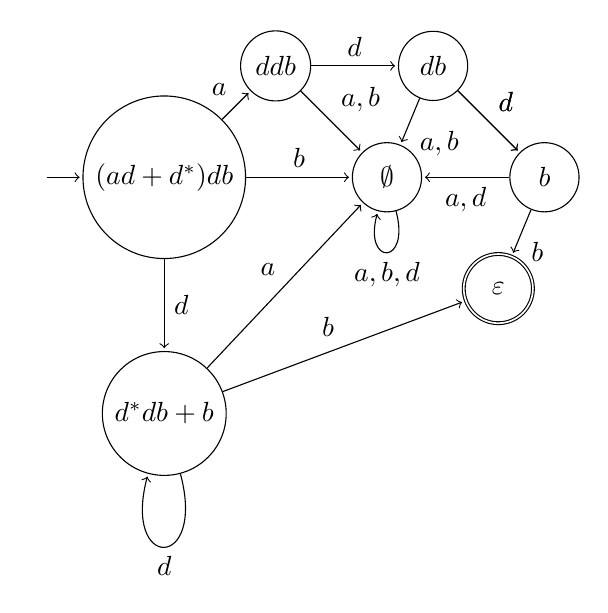
\begin{tikzpicture}[shorten >=1pt,node distance=2cm,on grid, auto,initial text=]
		\node[state,initial]	(q_0)												{$(ad+d^*)db$};
		\node[state]			(q_1)	[above right=of q_0]						{$ddb$};
		
		\node[state]			(q_3)	[right=of q_1]								{$db$};
		\node[state]			(q_4)	[below right=of q_3]						{$b$};
		\node[state]			(q_5)	[below right=of q_1]						{$\emptyset$};
		\node[state, accepting]	(q_6)	[below right=of q_5]						{$\varepsilon$};
		
		\node[state]			(q_2)	[below=30mm of q_0]							{$d^*db + b$};
		
		\path[->]	(q_0)	edge	node				{$a$}	(q_1)
							edge	node				{$d$}	(q_2)
							edge	node				{$b$}	(q_5)
					(q_1)	edge	node				{$d$}	(q_3)
							edge	node				{$a,b$}	(q_5)
					(q_2)	edge	node				{$a$}	(q_5)
							edge 	[loop below]	node	{$d$}	()
							edge	node				{$b$}	(q_6)
					(q_3)	edge	node				{$d$}	(q_4)
							edge	node				{$a,b$}	(q_5)
							edge	node				{$d$}	(q_4)
					(q_4)	edge	node				{$b$}	(q_6)
							edge	node				{$a,d$}	(q_5)
					(q_5)	edge	[loop below]	node	{$a,b,d$} ();
	\end{tikzpicture}
	\caption{Diagram of a Brzozowki DFA for the regular expression $(ad+d^*)db$.}
	\label{fig:brzozowski_derivatives_example}
\end{figure}

%This method can, however, lead to an exponential number of distinct derivatives in the worst case. Therefore, simplification rules and expression equivalences are critical to making the approach practical.

%\subsection{Antimirov's Partial Dertivatives}
%Proposed by Valery Antimirov in 1996 \cite{pdregex_antimirov}, the partial derivatives construction generalizes Brzozowski's derivatives to build an NFA rather than a DFA. Instead of producing a single derivative for each symbol, Antimirov's method produces a \emph{set} of partial derivatives, reflecting the inherent nondeterminism of the regular expression.
%
%This construction avoids $\varepsilon$-transitions and yields a compact $\varepsilon$-free NFA. Each partial derivative corresponds to a transition in the automaton, and the process naturally handles alternation and repetition.
%
%\begin{defn}[Partial Derivatives Automaton]
%	Let $\alpha \in RegExp$ over $\Sigma$. The partial derivatives automaton for $\alpha$ is defined as the non-deterministic finite automaton $\mathcal{N} = (Q_{\mathcal{PD}}, \Sigma, q_0, \delta, F)$. $q_0$ is the initial state and belongs to the set of states $Q_{\mathcal{PD}}$. It is important to note that $q_0 = \alpha$. The transition function is defined as $\delta(q,a) = \partial_a(q)$ for all symbols $a \in \Sigma$ and states $q \in Q_{\mathcal{PD}}$. The set of final states is defined as $F = \{ q \in Q_{\mathcal{PD}} \, | \, \varepsilon(q) = \varepsilon \}$.
%\end{defn}
%
%Recalling from \ref{chap:prelim:linear_form}, the linear form can be used as an efficient way to compute partial derivatives.
%Let $\alpha \in RegExp$ over $\Sigma$ and $a \in \Sigma$:
%\begin{centering}
%	$\delta(\alpha, a) = \{  \}$
%\end{centering}

\subsection{Antimirov's Partial Derivatives}
Proposed by Valery Antimirov in 1996 \cite{pdregex_antimirov}, the partial derivatives construction generalizes Brzozowski's derivatives to build an NFA rather than a DFA. Instead of producing a single derivative for each symbol, Antimirov's method produces a \emph{set} of partial derivatives, reflecting the inherent nondeterminism of the regular expression.

This construction avoids $\varepsilon$-transitions and yields a compact $\varepsilon$-free NFA. Each partial derivative corresponds to a transition in the automaton, and the process naturally handles alternation and repetition.


\begin{defn}[Partial Derivatives Automaton]
	Let $\alpha \in RegExp$ over $\Sigma$. The partial derivatives automaton for $\alpha$ is defined as the non-deterministic finite automaton $\mathcal{N} = (Q_{\mathcal{PD}}, \Sigma, q_0, \delta, F)$. $q_0$ is the initial state and belongs to the set of states $Q_{\mathcal{PD}}$. It is important to note that $q_0 = \alpha$. The transition function is defined as $\delta(q,a) = \partial_a(q)$ for all symbols $a \in \Sigma$ and states $q \in Q_{\mathcal{PD}}$. The set of final states is defined as $F = \{ q \in Q_{\mathcal{PD}} \, | \, \varepsilon(q) = \varepsilon \}$.
\end{defn}

Recalling from \ref{chap:prelim:linear_form}, the linear form can be used as an efficient way to compute partial derivatives.
Let $\alpha \in RegExp$ over $\Sigma$ and $a \in \Sigma$:
\[
\delta(\alpha, a) = \partial_a(\alpha) = \{ \beta \mid (a,\beta) \in lf(\alpha) \}.
\]

That is, to compute the set of partial derivatives of $\alpha$ with respect to a symbol $a$, one inspects the linear form of $\alpha$ and collects all continuations $\beta$ that follow an $a$ in the prefix position. This characterization is not only concise but also algorithmically useful: it gives a direct recipe for building the transition relation of the partial derivatives automaton.

\begin{thm}[\cite{pdregex_antimirov}]
	For every regular expression $\alpha$, the partial derivatives automaton $\mathcal{N}_\alpha$ accepts exactly the language $L(\alpha)$. Moreover, the number of states of $\mathcal{N}_\alpha$ is bounded by $|\alpha|+1$.
\end{thm}

%For instance, let $\alpha = (ad+d^*)db$ over $\Sigma = \{a,b,d\}$. The set of 


\subsection{Position Automata}
%https://www.dcc.fc.up.pt/~nam/resources/publica/dlt16.pdf

% To first recall the notion of \emph{position automata} (also known as \emph{Glushkov automata}), one must first understand the idea of marking each occurrence of a symbol in a regular expression with a unique position. This transforms a regular expression into a \emph{marked regular expression}, where each letter is indexed according to its position in the expression when read left to right. The position automaton is then constructed from this marked version by associating each position with a distinct state, and defining transitions based on the structural analysis of the expression.

The \emph{position automaton}, also known as the \emph{Glushkov automaton}, is a type of $\varepsilon$-free nondeterministic finite automaton (NFA) constructed directly from a regular expression. Unlike the standard Thompson construction, which introduces $\varepsilon$-transitions that must later be eliminated, the Glushkov construction yields an automaton in which each state corresponds uniquely to a symbol occurrence---or \emph{position}---in the expression. \cite{mesh-of-automata}

Given a regular expression $E$, the Glushkov automaton $M_E$ is defined based on three key position-based functions:

\begin{itemize}
    \item \textbf{first$(E)$}: the set of positions that can appear first in some word of the language $\mathcal{L}(E)$.
    \item \textbf{last$(E)$}: the set of positions that can appear last in some word of $\mathcal{L}(E)$.
    \item \textbf{follow$(E, x)$}: for each position $x$, the set of positions that can immediately follow $x$ in some word of $\mathcal{L}(E)$.
\end{itemize}

To distinguish different occurrences of the same symbol, the construction introduces marked symbols. For example, the expression $(a + b)^*a(b + a)^*$ is rewritten as $(a_1 + b_2)^*a_3(b_4 + a_5)^*$. Each marked symbol corresponds to a unique position and becomes a distinct state in the automaton.

The Glushkov automaton $M_E = (Q, \Sigma, \delta, q_0, F)$ is constructed as follows:

\begin{itemize}
    \item $Q$ is the set of positions in $E$ (i.e., the marked symbols), plus an initial state $q_0$.
    \item For each symbol $a \in \Sigma$:
    \begin{itemize}
        \item $\delta(q_0, a) = \{ x \in \text{first}(E) \mid \text{symbol}(x) = a \}$
        \item $\delta(x, a) = \{ y \in \text{follow}(E, x) \mid \text{symbol}(y) = a \}$
    \end{itemize}
    \item The set of final states $F$ is $\text{last}(E)$; if $\varepsilon \in \mathcal{L}(E)$, then $q_0$ is also final.
\end{itemize}

This automaton captures the structural flow of $E$ by tracing symbol sequences as state transitions. It is $\varepsilon$-free and has one state per symbol occurrence, which results in at most a quadratic number of transitions with respect to the size of $E$.

An important property of the Glushkov automaton is its relationship to unambiguity. A regular expression is \emph{weakly unambiguous} if and only if its Glushkov automaton is unambiguous, i.e., there exists at most one accepting path for each accepted word. This makes the Glushkov construction a practical and efficient tool in applications requiring unambiguous parsing, such as syntax analysis in document type definitions (e.g., SGML and XML DTDs).



% The key to this construction lies in the inductive computation of three sets: \emph{First}, \emph{Last}, and \emph{Follow}.The \emph{First} set contains positions that may begin a word in the language; the \emph{Last} set includes positions that may end such words; and the \emph{Follow} relation determines which positions can immediately follow a given position in any word generated by the expression. The resulting automaton has states corresponding to positions, transitions derived from the \emph{Follow} relation, an initial state representing position 0 (the start of matching), and final states determined by the \emph{Last} set, extended with position 0 if the empty string is accepted. \cite{mesh-of-automata}


\section{FAdo}
The FAdo \cite{fado_paper} project is an open-source implementation of several sets of tools for formal languages manipulation. In order to allow quick prototyping and testing of algorithms, these tools were developed in Python. Regular languages can be represented by regular expressions which are defined in \texttt{reex.py} - or by finite automata which are defined in \texttt{fa.py}.

\subsection{Finite Automata}

\begin{figure}[H]
	\centering
	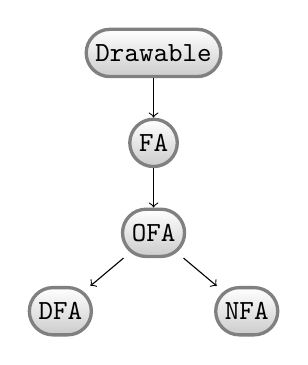
\begin{tikzpicture}[node distance=5mm,
		terminal/.style={
			% The shape:
			rectangle,minimum size=6mm,rounded corners=3mm,
			% The rest
			very thick,draw=black!50,
			top color=white,bottom color=black!20,
			font=\ttfamily}]
		\node (c_dwble)		[terminal]                {Drawable};
		\node (c_fa)		[terminal, below=of c_dwble]   {FA};
		\node (c_ofa)		[terminal, below=of c_fa] {OFA};
		\node (c_nfa)		[terminal, below right=of c_ofa] {NFA};
		\node (c_dfa)		[terminal, below left=of c_ofa]{DFA};
		
		\path	(c_dwble)	edge[->]	(c_fa)
				(c_fa)		edge[->]	(c_ofa)
				(c_ofa)		edge[->]	(c_dfa)
							edge[->]	(c_nfa);
	\end{tikzpicture}
	\caption{Class inheritance organization in FAdo's finite automata code file, \texttt{fa.py} (excluding the \texttt{SemiDFA} class)}
	\label{fig:fado_fa_diag}
\end{figure}

%As shown in \ref{fig:fado_fa_diag}, \texttt{FAdo}'s FA implementation utilizes the base class \texttt{Drawable} all the other children classes. The \texttt{Drawable} class will only set up some basic methods and properties used to draw the automata with the help of the \texttt{graphviz} library.
%The \textt{}


As shown in Figure~\ref{fig:fado_fa_diag}, FAdo organizes its implementation of finite automata as an inheritance hierarchy. At the top level, the class \texttt{Drawable} provides only drawing functionality, relying on the \texttt{graphviz} backend to visualize automata.

On top of this, the class \texttt{FA} defines the abstract interface for finite automata, introducing the fundamental components: the set of states, the alphabet, the transition function, the initial state(s), and the set of final states. This class also establishes common methods for manipulating these elements and for interoperability between automata.

The class \texttt{OFA} (``one-way finite automaton'') specializes \texttt{FA} and serves as the immediate superclass for concrete models. It defines abstract operations such as evaluation of symbols, addition of transitions, and access to useful states, ensuring a consistent contract across different automaton types.

Two subclasses will then inherit from \texttt{OFA}:
\begin{itemize}
	\item \texttt{NFA} --- implements nondeterministic finite automata, possibly with $\varepsilon$-transitions. It provides methods for epsilon-closure, elimination of $\varepsilon$-moves, subset construction into a DFA, and regular operations such as union, concatenation, and Kleene star.
	\item \texttt{DFA} --- implements deterministic finite automata. It enforces determinism by construction and provides efficient word evaluation and minimization routines.
\end{itemize}

\subsection{Regular Expressions}
In \texttt{reex.py}, FAdo defines the \texttt{RegExp} base class for all regular expressions, declaring therein a class variable \texttt{sigma}, formally known as the set of symbols ($\Sigma$).
To represent any and all base constructions of a regular expressions, FAdo defines base classes for each of them:
\begin{itemize}
    \item \textbf{CEmptySet}: The empty symbol set. ($\emptyset$)
    \item \textbf{CEpsilon}: The empty string. ($\varsigma$)
    \item \textbf{CAtom}: A simple symbol. (e.g. $'a'$)
    \item \textbf{CDisj}: The $+$ operation between symbols. (e.g. \texttt{CDisj(CAtom(a),CAtom(b))} represents the regular expression $R=a+b$ where $a,b \in \Sigma_R$)
    \item \textbf{CConcat}: The $\cdot$ operation 
    \item \textbf{CStar}: The Kleene closure over a set of symbols (e.g. \texttt{CStar(CDisj(CAtom(a),CAtom(b)))} representes the regular expression $R=(a+b)^*$ where $a,b \in \Sigma_R$)

\end{itemize}

In order to parse expressions into FAdo's classes and types, \emph{lark} was used. \emph{lark} is a parsing toolkit for Python. It can parse all context-free languages.





%\chapter{Estado da Arte}\label{chap:stat}
% \chapter{Estado da Arte}\label{chap:stat}

Sem conteúdo relevante, apenas com texto para ocupar o espaço.

\section{Section example}
\lipsum[1-6]
\section{Second Section example}
\subsection{SubSection example}
\lipsum[7-10]


\chapter{State of the Art}\label{chap:art}

\section{Overview of XYZ}
%%%%%%%%%%%%%%%%%%%%%%%%%%%%%%%%%%%%%%%%
Computers are devices that



%\chapter{Desenho da Arquitetura}\label{chap:syst}
\chapter{Counting}\label{chap:counting}
In this chapter, we will explore the concept of counting in the context of formal languages and automata theory as well as explain the implementation for fixed and bounded repetition in FAdo.

\section{Counting in Formal Languages}
In formal language theory, counting refers to the ability of a language or an automaton to enforce numeric constraints over the number of symbols or patterns within strings. Specifically, it deals with the ability to recognize whether certain elements occur a specified number of times—or in a specific numerical relationship to others.
Current tools are already able to do this, including some non-backtracking matchers. However, even for tools based on NFA and DFA, these operators are problematic due to the complexity of their manipulation. The aim of the work here described is to build derivative-based tools that may be more efficient and/or secure. 

\section{Derivatives of fixed and bounded repetition operators} %TODO: CHANGE THIS
Given a word $w$ and a regular expression $e$, $w \in L(e)$ if $\varepsilon(d_w(e)) = \varepsilon$.
In order to match with fixed and bounded repetition using derivatives, one must first define them for those operations.

\begin{thm}
	Given $e \in RegExp(\Sigma)$, the following holds:
	\begin{align*}
		\varepsilon(e) + e = e
	\end{align*}
\end{thm}
\begin{proof}
	Let $e \in RegExp(\Sigma)$. The proof considers the cases where $\varepsilon \in L(e)$ and $\varepsilon \notin L(e)$.
	For $\varepsilon \in L(e)$, we have that $\varepsilon(e) = \varepsilon$. And then,
	\begin{align*}
		& \varepsilon(e) + e = e \\
		& \Rightarrow \varepsilon + e = e \\
		& \Rightarrow e = e
	\end{align*}
	holds. On the other hand, for $\varepsilon \notin L(e)$, we have that $\varepsilon(e) = \emptyset$. Therefore,
	\begin{align*}
		& \varepsilon(e) + e = e \\
		& \Rightarrow \emptyset + e = e \\
		& \Rightarrow e = e
	\end{align*}
	also holds.
\end{proof}

\subsection{Fixed Repetition}
%For a fixed repetition, we need $r$ to occur $n$ times, resulting in the notion $r^n$.

% PROOF
%\begin{thm}
%	Given $e \in RegExp(\Sigma)$ and $n \in \Npos$, we have that
%	\begin{align*}
%		d_a(e^n) = d_a(e)e^{n-1}
%	\end{align*}
%	is true.
%\end{thm}
%\begin{proof}
%	Let $e \in RegExp(\Sigma)$ and $n \in \Npos$. The following holds:
%	\begin{align*}
%		d_a(e) = d_a(e)e^0 = d_a(e)
%	\end{align*}
%	We can also suppose that
%	\begin{align*}
%		d_a(e^{n-1}) = d_a(e)e^{n-2}
%	\end{align*}
%	And so, we can use the results above to do the following:
%	\begin{align*}
%		d_a(e^n) &= d_a(ee^{n-1}) \\
%		&= d_a(e)e^{n-1} + \varepsilon(e)d_a(e^{n-1}) \\
%		&= d_a(e)e^{n-1} + \varepsilon(e)d_a(e)e^{n-2} \\
%		&= (d_a(e)e + \varepsilon(e)d_a(e))e^{n-2} \\
%		&= (d_a(e)(e+\varepsilon(e)))e^{n-2} \\
%		&= d_a(e)e^{n-1}
%	\end{align*}
%\end{proof}
\begin{thm}
	\label{thm:fixed_repetition_derivative}
	Given $e \in RegExp(\Sigma)$ and $n \in \Npos$, we have:
	\begin{align*}
		d_a(e^n) = d_a(e)\,e^{n-1}.
	\end{align*}
\end{thm}

\begin{proof}
	We proceed by induction on $n \in \Npos$. For the base case \( n = 1 \),
	\begin{align*}
		d_a(e^1) = d_a(e) = d_a(e)e^0 = d_a(e)\varepsilon = d_a(e).
	\end{align*}
	Since the identity holds for \(n = 1\), lets assume that the identity holds for some \(n-1 \geq 1\), i.e.,
	\begin{align*}
		d_a(e^{n-1}) = d_a(e)e^{n-2}.
	\end{align*}
	We want to show it holds for \(n\). Using the product rule:
	\begin{align*}
		d_a(e^n) &= d_a(ee^{n-1}) \\
		&= d_a(e) e^{n-1} + \varepsilon(e) d_a(e^{n-1}) \\
		&= d_a(e) e^{n-1} + \varepsilon(e) d_a(e) e^{n-2} \\
		&= d_a(e) \left(e^{n-1} + \varepsilon(e) e^{n-2}\right) \\
		&= d_a(e) \left(ee^{n-2} + \varepsilon(e) e^{n-2}\right) \\
		&= d_a(e) (e + \varepsilon(e))e^{n-2} \\
		&= d_a(e) e^{n-1}.
	\end{align*}
	This completes the induction.
\end{proof}

As an example, let $e = ab$ such that $e^2 = abab$. Using the theorem above:
\begin{align*}
	d_a(e^2) &= d_a(e)e \\
	&= d_a(ab)ab  \\
	&= bab
\end{align*}

% ADD e^n results for n=0, n=1 and n>1

We can also define partial derivatives and the linear form for this new operator. We have
\begin{gather*}
	\partial_a(e^n) = \partial_a(e)e^{n-1} \\
	lf(e^n) = lf(e)e^{n-1}
\end{gather*}
for $e \in RegExp(\Sigma)$, $a \in \Sigma$, and $n \in \Npos$.

\subsection{Bounded Repetition}
%Supplementing the fixed repetition notion, we now add a maximum bound so that $r$ can occur at least $n$ times and at maximum $m-1$ times: $r^{n,m}$.

\begin{thm}
	Given $e \in RegExp(\Sigma)$, $n \in \Npos$, $m > n$, and $a \in \Sigma$, we have:
	\begin{align*}
		d_a(e^{n,m}) =
		\begin{cases}
			d_a(e) e^{n-1,m-1}, & \text{if } n > 1, \\
			d_a(e) + d_a(e) e^{1,m-1}, & \text{if } n = 1.
		\end{cases}
	\end{align*}
\end{thm}

\begin{proof}
	Let $e \in RegExp(\Sigma)$ and let $n, m \in \Npos$ with $m > n$. By definition of bounded iteration:
	\begin{align*}
		e^{n,m} &= \sum_{i=n}^{m} e^i,
	\end{align*}
	and by the linearity of derivatives over sums:
	\begin{align*}
		d_a(e^{n,m}) &= \sum_{i=n}^{m} d_a(e^i).
	\end{align*}
	Using the known identity $d_a(e^i) = d_a(e) e^{i-1}$, we have:
	\begin{align*}
		d_a(e^{n,m}) &= \sum_{i=n}^{m} d_a(e) e^{i-1} \\
		&= d_a(e) \sum_{i=n}^{m} e^{i-1}.
	\end{align*}
	Letting $j = i - 1$, this becomes:
	\begin{align*}
		d_a(e^{n,m}) &= d_a(e) \sum_{j=n-1}^{m-1} e^j = d_a(e) e^{n-1,m-1}.
	\end{align*}
	Considering both cases, for $n > 1$, the expression is already in its final form:
	\begin{align*}
		d_a(e^{n,m}) = d_a(e) e^{n-1,m-1}.
	\end{align*}
	And for $n = 1$, we have:
	\begin{align*}
		d_a(e^{1,m}) &= d_a(e) e^{0,m-1} \\
		&= d_a(e) + d_a(e) e^{1,m-1}.
	\end{align*}
	This completes the proof.
\end{proof}
Furthermore, we can include the infinite upper bound: $e^{n,\infty}$.
\begin{align*}
	e^{n,\infty} = e^ne^\star
\end{align*}
We can simplify it even more, depending on the value of $n$. Assuming $n=0$:
\begin{align*}
	e^{0,\infty} = e^0e^\star = \varepsilon e^\star =  e^\star
\end{align*}
Lastly, for $n=1$:
\begin{align*}
	e^{1,\infty} = e^1e^\star = ee^\star =  e^+
\end{align*}

These relations allow to substitute $r^\star$ and $r^+$ with counting expressions. However, in the \emph{FAdo} package, we consider also the classic iterators.

\begin{thm}
	Given $e \in RegExp(\Sigma)$, $n \in \N$ and $a \in \Sigma$, we have:
	\begin{align*}
		d_a(e^{n,\infty}) =
		\begin{cases}
			d_a(e)e^{n-1, \infty}, & \text{if } n>0, \\
			d_a(e)e^{0, \infty}, & \text{otherwise}.
		\end{cases}
	\end{align*}
\end{thm}
\begin{proof}
	Let $e \in RegExp(\Sigma)$, $n \in \N$, and $a \in \Sigma$. We have,
	\begin{align*}
		d_a(e^{n,\infty}) &= d_a(e^ne^\star) \\
		&= d_a(e^n)e^\star + \varepsilon(e)d_a(e)e^\star \\
		&= (d_a(e^n) + \varepsilon(e)d_a(e))e^\star \\
		&= (d_a(e)e^{n-1} + d_a(e) \varepsilon(e))e^\star \\
		&= (d_a(e)(e^{n-1} + \varepsilon(e)))e^\star \\
		&= d_a(e)e^{n-1}e^\star \\
		&= d_a(e)e^{n-1, \infty}.
%		&= d_a(e^n)e^\star. %\\
%		\intertext{using \ref{thm:fixed_repetition_derivative}:}
%		&= d_a(e)e^{n-1}e^\star
%	\end{align*}
%	Now, using \ref{thm:fixed_repetition_derivative}:
%	\begin{align*}
%		d_a(e^n)e^\star = d_a(e)e^{n-1}e^\star = d_a(e)e^{n-1, \infty}.
	\end{align*}
	Otherwise, if $n=0$, we can just replace accordingly:
	\begin{align*}
		d_a(e^ne^\star) = d_a(e^0e^\star) = d_a(e^\star) = d_a(e)e^\star = d_a(e)e^{0, \infty}.
	\end{align*}
	This concludes the proof.
\end{proof}
For instance, given $e = ab$ such that $e^2 = abab$ and $e^3 = ababab$, we have:
\begin{align*}
	d_a(e^{2,4}) &= d_a(e)e^{[1,3[} \\
	&= b(ab)^{[1,3[} \\
	&= bab + babab
%	d_a(r^{2,4}) &= d_a(abab) + d_a(ababab) \\
%	&= d_a(abab) + d_a(ababab) \\
%	&= d_a(a)bab + d_a(bab) + d_a(a)babab + d_a(babab) \\
%	&= \varepsilon bab + \emptyset + babab + \emptyset \\
%	&= bab + babab.
\end{align*}
Extending to the infinity case, $e^{2, \infty}$:
\begin{align*}
	d_a(e^{2, \infty}) &= d_a(e)e^{1, \infty} \\
	&= b(ab)e^{1,\infty} \\
	&= bab + b(ab)^+
%	d_a(r^{[2,\inf[}) &= d_a(abab) + d_a((ab)^*) \\
%	&= d_a(a)bab + d_a(bab) + d_a(ab)\cdot(ab)^* \\
%	&= \varepsilon bab + \emptyset + (d_a(a)b + d_a(b)) \cdot (ab)^* \\
%	&= bab + (\varepsilon b + \emptyset) \cdot (ab)^* \\
%	&= bab + b(ab)^*.
\end{align*}

Lastly, we can define the partial derivatives and linear form for these operators too.
We have for bounded repetition (excluding infinity cases),
\begin{align*}
	\partial_a(e^{n,m}) &= \begin{cases}
		\partial_a(e)e^{n-1,m-1}, & \text{if $n > 1$}, \\
		\partial_a(e) + \partial_a(e)e^{1,m-1}, & \text{if $n=1$}.
	\end{cases} \\
	lf_a(e^{n,m}) &= \begin{cases}
		lf_a(e)e^{n-1,m-1}, & \text{if $n > 1$}, \\
		lf_a(e) + lf_a(e)e^{1,m-1}, & \text{if $n=1$}.
	\end{cases} \\
\intertext{and for its infinity cases,}
	\partial_a(e^{j,\infty}) &= \begin{cases}
		\partial_a(e)e^{j-1, \infty}, & \text{if $j > 0$}, \\
		\partial_a(e)e^{0, \infty}, & \text{otherwise}.
	\end{cases} \\
	lf_a(e^{j,\infty}) &= \begin{cases}
		lf_a(e)e^{j-1, \infty}, & \text{if $j > 0$}, \\
		lf_a(e)e^{0, \infty}, & \text{otherwise}.
	\end{cases}
%	\partial_a(e^n) = \partial_a(e)e^{n-1} \\
%	lf(e^n) = lf(e)e^{n-1}
\end{align*}
for bounded repetition, with $e \in RegExp(\Sigma)$, $a \in \Sigma$, $n \in \Npos$, $m>n$, $j \in \N$.

%For instance, if $m = 2$, we have that $r^{[2, \inf[}$

%The regular expression $r^{[2, \inf[}$ will match any $(ab)^k$ with $k \geq 2$.

%Given $w = abababab$ and $m = 2$,  will match 

%The string $abababab$ can be matched by $r^{[2, \inf[}$

%\begin{thm}
%	Given $e \in RegExp(\Sigma)$, $n \in \Npos$ and $m>n$, we have that
%	\begin{align*}
%	%	d_a(e^{n,m}) = d_a(e) e^{n-1,m-1}
%	d_a(e^{n,m}) = \begin{cases}
%		d_a(e)e^{n-1,m-1} & n>1 \\
%		d_a(e)+(d_a(e))e^{1,m-1} & n=1
%	\end{cases}
%	\end{align*}
%	is true.
%\end{thm}
%\begin{proof}
%	Let $e \in RegExp(\Sigma)$. We first need to simplify the main expression:
%	\begin{align*}
%		d_a(e^{n,m}) &= \sum_{i=n}^{m} d_a(e^i) \\
%		&= \sum_{i=n}^{m} (d_a(e))e^{i-1} \\
%		&= d_a(e) \sum_{j=n-1}^{m-1} e^j \\
%		&= d_a(e) e^{n-1,m-1}
%	\end{align*}
%	Thus, for $n=1$, we have that
%	\begin{align*}
%		d_a(e^{n,m}) &= d_a(e)e^{0,m-1} \\
%		&= d_a(e) + (d_a(e))e^{1,m-1}
%	\end{align*}
%	And lastly, for $n>=1$ we have that
%	\begin{align*}
%		d_a(e^{n,m}) &= (d_a(e))e^{n-1,m-1}
%	\end{align*}
%\end{proof}

%For instance, if $m = 2$, we have that $r^{[2, \inf[}$

%The regular expression $r^{[2, \inf[}$ will match any $(ab)^k$ with $k \geq 2$.

%Given $w = abababab$ and $m = 2$,  will match 

%The string $abababab$ can be matched by $r^{[2, \inf[}$


\section{Implementation in FAdo}
In order to implement these new syntactic constructs of extended regular expressions in FAdo, we added exact-power and counted-repetition nodes to the regular expression abstract syntax tree and define their derivatives, partial derivatives and linear form cases.

\subsection{CPower}
\textit{CPower} is the class responsible for the construction of regular expressions using the fixed repetition operator.

\begin{lstlisting}[language=Python]
class CPower(Unary):
	def __init__(self, arg, n, sigma=None):
	self.arg = arg
	self.n = n
	self.Sigma = sigma
	self._ewp = False if self.n > 0 else True
	
	...
\end{lstlisting}

As shown above, the class inherits from the \textit{Unary} class, which only defines the \textit{Unary.Sigma} and \textit{Unary.arg} properties, letting the class hold a alphabet set (representing $\Sigma$) and the symbol used to construct this operator.
In order to integrate \textit{CPower} fully with \textit{FAdo}, some more methods had to be implemented.

\begin{lstlisting}[language=Python]
	def linearForm(self):
		arg_lf = self.arg.linearForm()
		lf = dict()
		for head in arg_lf:
			lf[head] = set()
			for tail in arg_lf[head]:
				lf[head].add(self.derivative(head))
		return lf

	def partialDerivatives(self, sigma):
		return self.arg.partialDerivatives(sigma)
	
	def derivative(self, sigma):
		if str(sigma) in str(self.Sigma):
			if self.n == 0:
				return CEmptySet(sigma)
			elif self.n == 1:
				return self.arg.derivative(sigma)
			else:
				return CConcat(self.arg.derivative(sigma), CPower(self.arg, self.n-1, self.Sigma))
		else:
			return CEmptySet(sigma)
\end{lstlisting}

\subsection{CCount}
\textit{CCount} is the class responsible for the construction of regular expressions using the bounded repetition operator.


\begin{lstlisting}[language=Python]
	class CCount(Unary):
		def __init__(self, arg, min, max = None, sigma = None):
			self.arg = arg
			self.min = int(min)
			self.max = "inf" if max == -1 or max == "inf" else int(max)-1
			self.Sigma = sigma
	
			if self.min==0:
				self._ewp = True
\end{lstlisting}

As shown above, and much like \textit{CPower}, the class also inherits from \textit{Unary}. The constructor adjusts the bounds accordingly and sets the empty word property based on whether the minimum repetition is zero.

To fully integrate the class with \textit{FAdo}, several methods are implemented, including string representation, partial derivatives, linear form computation, and marking functions:

\begin{lstlisting}[language=Python]
	def derivative(self, sigma):
		if str(sigma) in str(self.Sigma):
			if self.max == "inf" or self.max == None:
				if self.min == 0:
					return CConcat(self.arg.derivative(sigma), CStar(self.arg, self.Sigma))
				else:
					return CConcat(self.arg.derivative(sigma), CCount(self.arg, self.min-1, self.max, sigma), self.Sigma)
			else:
				if self.max > 1:
					if self.min == 0:
						return CConcat(self.arg.derivative(sigma), CCount(self.arg, self.min, int(self.max), self.Sigma))
					else:
						return CConcat(self.arg.derivative(sigma), CCount(self.arg, self.min-1, int(self.max), self.Sigma))
				elif self.max == 1:
					return self.arg.derivative(sigma)
				else:
					CEpsilon(sigma)
		else:
			return CEmptySet(sigma)
		
	def partialDerivatives(self, sigma):
		arg_pdset = self.arg.partialDerivatives(sigma)
		pds = set()
		for pd in arg_pdset:
			if pd.emptysetP():
				pds.add(CEmptySet(self.Sigma))
			elif pd.epsilonP():
				pds.add(self)
			else:
				pds.add(CConcat(pd, self, self.Sigma))
		return pds
\end{lstlisting}

The \texttt{linearForm} method is exactly the same as \texttt{CPower}'s.

%\begin{lstlisting}[language=Python]
%	def linearForm(self):
%		arg_lf = self.arg.linearForm()
%		lf = dict()
%		for head in arg_lf:
%			lf[head] = set()
%			for tail in arg_lf[head]:
%				lf[head].add(self.derivative(head))
%		return lf
%\end{lstlisting}

\subsection{Grammar}
For ease of use and protoyping, we utilized \textit{FAdo}'s ability to parse a regular expression using a common Python \textit{string}. To do this, \textit{FAdo} utilizes a library called Lark. Lark is a modern, fast and flexible parsing toolkit for Python that supports both LALR(1) and Earley parsers, enabling the parsing of all context-free grammars with features like EBNF, AST generation, and grammar composition \cite{lark_parser}.
The new grammar can be seen in Appendix~\ref{appendix:regexp_lark} and the most notable changes are the following:
\begin{lstlisting}
	| rep _CARET _LEFBR digit _RIGBR -> pow_min
	| rep _CARET _LEFBR digit _COMMA digit _LEFBR -> pow_minmax
	| rep _CARET _LEFBR digit _COMMA _INFTY _LEFBR -> pow_inf
\end{lstlisting}
These rules (along with some more utilitary definitions such as the \texttt{\_LEFBR} and \texttt{\_RIGBR}, which are the symbols '\texttt{\string[}' and '\texttt{\string]}') will route the following cases (code in Appendix~\ref{appendix:regexp_builders}):
\begin{itemize}
	\item \textbf{pow\_min}: For the cases $e^{n}$ and $e^{n,\infty}$, where $e \in RegExp(\Sigma)$ and $n \in \Npos$
	\item \textbf{pow\_minmax}: For the case $e^{n,m}$, where $e \in RegExp(\Sigma)$ and $n \in \Npos, m>n$
	\item \textbf{pow\_inf}: Calls \textit{pow\_min} with a special argument that selects the infinity case
\end{itemize}

\subsection{Matching}
To demonstrate how matching is performed using the implemented operators, we can consider a concrete example.
For instance, let $r = (ab)^{1,3}$. The following code snippet shows how this expression can be parsed, transformed into an internal representation, and converted into a DFA using Brzozowski's construction:
%In order to match using these implemented notions, we can do as follows. . We can parse the regular expression and display it like so:
\begin{lstlisting}[language=Python]
	r = "(ab)^[1,3["
	tree = regGrammar.parse(r)
	reg : RegExp = BuildRegexp(context={"sigma": None}).transform(tree)
	reg.setSigma(reg.setOfSymbols())
	dfa_z = reg.dfaBrzozowski()
	dfa_z.display()
\end{lstlisting}

\begin{figure}[H]
	\centering
	\begin{tikzpicture}[shorten >=1pt,node distance=2cm,on grid, auto,initial text=]
		
		% --- States ---
		\node[state, initial] (q0) {0};
		\node[state]          (q1) [above right=of q0] {1};
		\node[state]          (q2) [below right=of q0] {2};
		\node[state, accepting]         (q3) [right=22mm of q1] {3};
		\node[state]          (q4) [right=22mm of q2] {4};
		\node[state]          (q5) [above right=of q3] {5};
		\node[state]          (q6) [right=20mm of q3] {6};
		\node[state, accepting]         (q7) [right=22mm of q6] {7};
		\node[state]          (q8) [right=22mm of q7] {8};
		
		% --- Transitions ---
		\path[->]
		(q0) edge node {$b$} (q1)
		edge[swap] node {$a$} (q2)
		
		(q1) edge[loop above] node {$b, a$} ()
		
		(q2) edge node {$b$} (q3)
		edge[swap] node {$a$} (q4)
		
		(q4) edge[loop below] node {$b, a$} ()
		
		(q3) edge node {$b$} (q5)
		edge[swap] node {$a$} (q6)
		
		(q5) edge[loop above] node {$b, a$} ()
		
		(q6) edge node {$b$} (q7)
		edge[bend right=40, swap] node {$a$} (q8)
		
		(q7) edge node {$b, a$} (q8)
		
		(q8) edge[loop right] node {$b, a$} ();
	\end{tikzpicture}
	\caption{Diagram of the DFA built using Brzozowski's method for the regular expression $r = (ab)^{1,3}$.}
	\label{fig:dfa_brzozowski_counting}
\end{figure}


Then, try to match $w = ab$ using the same code from the snippet~\ref{code:eval_word_dfa}, which yields the following:
\begin{lstlisting}[language=Python]
	w belongs to the language of r
\end{lstlisting}
Trying again with a text that does not match, $w = ababab$, yields:
\begin{lstlisting}[language=Python]
	w does not belong to the language of r
\end{lstlisting}
%Formally, .

%\chapter{Desenvolvimento}\label{chap:dese}
\chapter{Matching}\label{chap:matching}
% Matching is used to search, validate, or extract parts of text based on these patterns. For example, a regex can be used to find all dates in a document or to ensure a password meets certain rules.

\emph{Matching} is the process of checking whether a piece of text fits a specific pattern described using a regular expression (regex).
In this chapter, we will discuss the different approaches to matching regular expressions, the implications of using them, and the performance considerations that arise from these choices. Furthermore, we will also present a novel approach based on a modified position automata, which aims to mitigate the performance issues associated with traditional regex engines while preserving some of the extended expressiveness of regex patterns.

\section{Overlapped versus Non-Overlapped Matching}
\label{sec:overlap-vs-nonoverlap}

In the context of regular expression matching, two distinct paradigms exist: \emph{overlapped matching} and \emph{non-overlapped matching}. Understanding their differences is crucial when designing matching engines, especially when completeness or performance is a concern.

\subsection*{Overlapped Matching}
Overlapped matching refers to finding all possible matches of a pattern in an input string. This is typically achieved by attempting a match starting at every index of the input. It is more exhaustive and useful in domains where no potential match should be missed, such as bioinformatics (DNA pattern searching).

For example, the indexed string $w = a_0 a_1 a_2 a_3$, when matched against using the pattern $aa$, will yield the following matched substrings:

\begin{itemize}
	\item $w_{[0,2[} = {\color{red}{aa}}aa$
	\item $w_{[1,3[} = a{\color{red}{aa}}a$
	\item $w_{[2,4[} = aa{\color{red}{aa}}$
\end{itemize}

\subsection*{Non-Overlapped Matching}
Non-overlapped matching (also referred to as \emph{disjoint}, \emph{standard}, or in some engines, \emph{greedy} matching) finds matches sequentially from left to right, and once a match is found, it advances the input pointer beyond the match. Unlike overlapped matchers, where overlapping is a feature by default, greedy matchers will often depend on the lookahead assertions to do so.

Using the same pattern $aa$ on $w = a_0 a_1 a_2 a_3$, a non-overlapped matcher may return:

\begin{itemize}
	\item $w_{[0,2[} = {\color{red}{aa}}aa$
	\item $w_{[2,4[} = aa{\color{red}{aa}}$
\end{itemize}

To summarize, overlapped matching provides a more complete view of potential matches, but at a higher computational cost. It is particularly well-suited to automata-based approaches like the modified position automaton described in this work.


\section{Modified Position Automata}
A \emph{position automaton} is a type of nondeterministic finite automaton (NFA).
We can enable overlapped matching by modifying the position automaton's construction using the algorithm described on  \ref{alg:nfaPosCount}.

\begin{algorithm}[H]
\caption{\textsc{nfaPosCount}($R$): Construct Special Position Automaton}
\label{alg:nfaPosCount}
\begin{small}
\begin{algorithmic}[1]
\Require Regular expression $R$
\Ensure NFA $A$

\State $A \gets$ new empty NFA
\State $i \gets A.\text{addInitialState}()$
\State $A.\text{addTransitionStar}(i, i)$ \Comment{Accept any symbol from $\Sigma$}

\State $f_R \gets R.\text{marked}()$
\State $\text{stack} \gets$ empty stack
\State $\text{addedStates} \gets$ empty map

\ForAll{$p \in First(f_R)$}
    \State $q \gets A.\text{addState}(p)$
    \State $\text{addedStates}[p] \gets q$
    \State $\text{stack}.\text{push}((p, q))$
    \State $A.\text{addTransition}(i, p, q)$
\EndFor

% \State $\text{FollowSets} \gets Follow(f_R)$

\While{stack is not empty}
    \State $(s, s_{\text{idx}}) \gets \text{stack}.\text{pop}()$
    \ForAll{$t \in Follow(f_R, s)$}
        \If{$t \in \text{addedStates}$}
            \State $q \gets \text{addedStates}[t]$
        \Else
            \State $q \gets A.\text{addState}(t)$
            \State $\text{addedStates}[t] \gets q$
            \State $\text{stack}.\text{push}((t, q))$
        \EndIf
        \State $A.\text{addTransition}(s_{\text{idx}}, t, q)$
    \EndFor
\EndWhile

\State $e \gets A.\text{addState}()$
\State $A.\text{addTransitionStar}(e, e)$

\ForAll{$p \in f_R.\text{Last}()$}
    \If{$p \in \text{addedStates}$}
        \State $A.\text{addFinal}(\text{addedStates}[p])$
        \State $A.\text{addTransitionStar}(\text{addedStates}[p], e)$
    \EndIf
\EndFor

\end{algorithmic}
\end{small}
\end{algorithm}

\section{Automata-Based Matching}

Given a regular expression $R$, one can construct an NFA $A$ such that $L(A) = L(R)$. Matching then reduces to verifying whether the automaton $A$ accepts the input string $s$. In DFA-based engines, each character of the input leads to a deterministic transition from one state to another, resulting in a guaranteed linear-time match. In contrast, NFA-based engines may involve branching paths due to nondeterminism and can require simulating multiple transitions concurrently.

% \section{Backtracking and Performance Implications}

% Many practical regular expression engines (such as those in Java, Perl, and Python) implement matching using \emph{backtracking}, which simulates an NFA by exploring all possible paths through the automaton recursively. While this allows support for rich and flexible patterns, it can introduce performance issues in certain cases. In particular, patterns with nested or ambiguous quantifiers may cause excessive backtracking, leading to exponential runtime in the worst case—a phenomenon known as \emph{regular expression denial of service} (ReDoS).

For example, consider the following regex pattern:
\begin{verbatim}
	^(a+)+$
\end{verbatim}

\section {Matching with the Modified Position Automaton}
One can find all matches over an input string by constructing the modified position automaton from a regular expression and then simulating the automaton's transitions over the input string. The algorithm presented in this section is designed to track the start and end positions of all matches, including overlapping ones, without relying on backtracking.

\begin{algorithm}[H]
\caption{\textsc{tableMatcher}$(A, s)$: Modified Position Automaton Multi-matcher}
\label{alg:table-matcher}
\begin{small}
\begin{algorithmic}[1]
\Require $A = (\Sigma, Q, \delta, I, F)$: NFA
\Require $s$: input string
\Ensure $M$: mapping from final states to lists of match positions

\State $symbols \gets$ list with $\varepsilon$ prepended to $s$
\State $currentRow \gets$ empty map from states to list of position pairs
\State $finalMatches \gets$ empty map from states to list of matches
\State $position \gets 0$

\ForAll{$sym$ in $symbols$}
    \If{$sym = \varepsilon$}
        \ForAll{$q_0 \in I$}
            \State $currentRow[q_0] \gets [(0, 0)]$
        \EndFor
    \Else
        \State $nextRow \gets$ empty map
        \If{$sym \in \Sigma$}
            \ForAll{$q \in$ \textbf{keys}($currentRow$)}
                % \State $transitions \gets \delta(q, sym)$
                \If{$|\delta(q, sym)| > 0$}
                    \ForAll{$q' \in \delta(q, sym)$}
                        \ForAll{$(start, \_) \in currentRow[q]$}
                            \If{$q' = q$ and $q' \in I$}
                                \State append $(position, position)$ to $nextRow[q']$
                            \Else
                                \State append $(start, position)$ to $nextRow[q']$
                                \If{$q' \in F$}
                                    \State append $(start, position)$ to $finalMatches[q']$
                                \EndIf
                            \EndIf
                        \EndFor
                    \EndFor
                \EndIf
            \EndFor
        \Else
            \Comment{Symbol not in $\Sigma$; treat as fresh start}
            \ForAll{$q_0 \in I$}
                \State $nextRow[q_0] \gets [(position, position)]$
            \EndFor
        \EndIf
        \State $currentRow \gets nextRow$
        \State $position \gets position + 1$
    \EndIf
\EndFor
\State \Return $finalMatches$
\end{algorithmic}
\end{small}
\end{algorithm}

\clearpage

As an example, consider the following regular expression $R$ and input string $w$:
\begin{center}
	$R = (aa+aaa)(aaa+aa)$ \break
	$w = aaaaabaaaaa$
\end{center}

We can separate $R$ into two matching groups:
\begin{itemize}
	\item The first group $(aa+aaa)$ will match either two or three $a$ symbols (e.g. $aaa$ will yield three overlapped matches: ${\color{red}{aa}}a$, $a{\color{red}{aa}}$ and ${\color{red}{aaa}}$).
	\item The second group $(aaa+aa)$ will also match either two or three $a$ symbols, much like the first group.
\end{itemize}



The Glushkov automaton construction for $R$ is as follows:

\begin{figure}[H]
	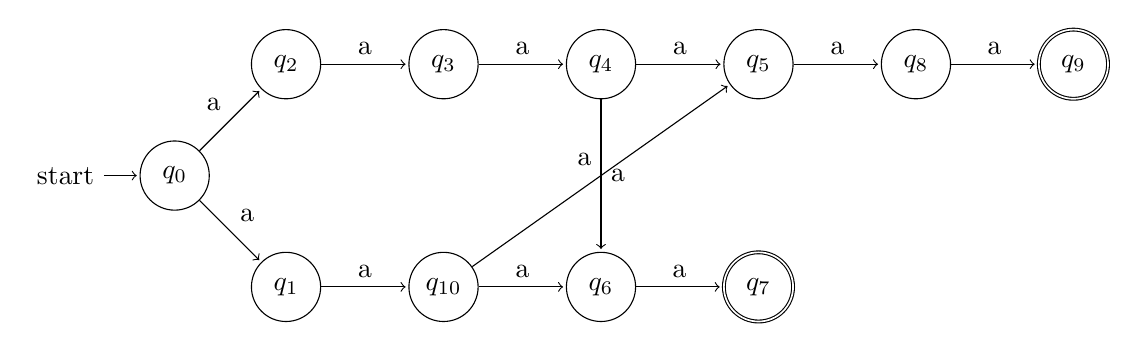
\begin{tikzpicture}[shorten >=1pt,node distance=2cm,on grid, auto]
		\node[state, initial] (q0) {$q_0$};
		\node[state] (q2) [above right=of q0] {$q_2$};
		\node[state] (q3) [right=of q2] {$q_3$};
		\node[state] (q4) [right=of q3] {$q_4$};
		\node[state] (q5) [right=of q4] {$q_5$};
		\node[state] (q8) [right=of q5] {$q_8$};
		\node[state,accepting] (q9) [right=of q8] {$q_9$};
		
		\node[state] (q1) [below right=of q0] {$q_1$};
		\node[state] (q10) [right=of q1] {$q_{10}$};
		\node[state] (q6) [right=of q10] {$q_6$};
		\node[state,accepting] (q7) [right=of q6] {$q_7$};
		
		\path[->]	(q0)	edge	node	{a} (q1)
		edge	node	{a} (q2)
		(q1)	edge	node	{a} (q10)
		(q10)	edge	node	{a} (q6)
		(q10)	edge	node	{a} (q5)
		(q6)	edge	node	{a} (q7)
		(q2)	edge	node	{a} (q3)
		(q3)	edge	node	{a} (q4)
		(q4)	edge	node	{a} (q5)
		(q4)	edge	node	{a} (q6)
		(q5)	edge	node	{a} (q8)
		(q8)	edge	node	{a} (q9);
	\end{tikzpicture}
	\caption{Default Glushkov automaton}
\end{figure}


Meanwhile, the modified position automaton for this regular expression can be constructed using the algorithm presented in \ref{alg:nfaPosCount}, resulting in the following:


\begin{figure}[H]
	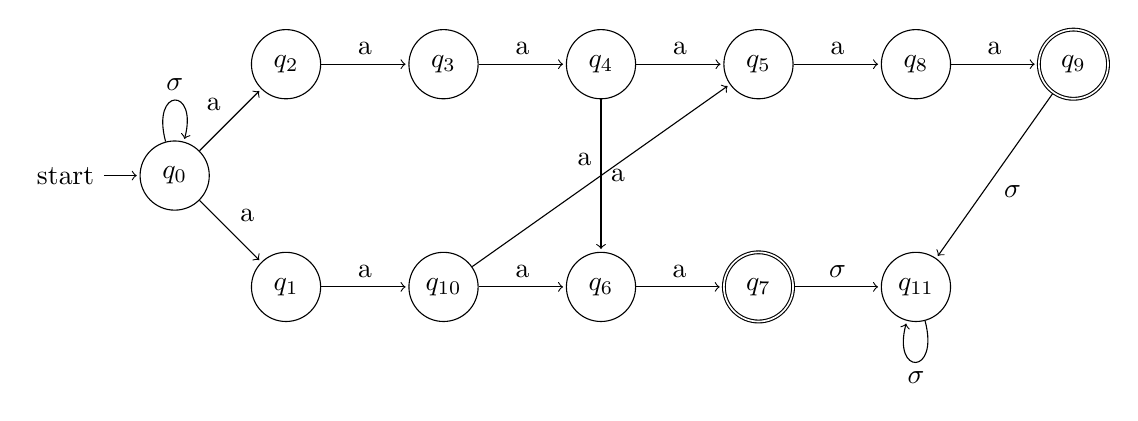
\begin{tikzpicture}[shorten >=1pt,node distance=2cm,on grid, auto]
		\node[state, initial] (q0) {$q_0$};
		\node[state] (q2) [above right=of q0] {$q_2$};
		\node[state] (q3) [right=of q2] {$q_3$};
		\node[state] (q4) [right=of q3] {$q_4$};
		\node[state] (q5) [right=of q4] {$q_5$};
		\node[state] (q8) [right=of q5] {$q_8$};
		\node[state,accepting] (q9) [right=of q8] {$q_9$};
		
		\node[state] (q1) [below right=of q0] {$q_1$};
		\node[state] (q10) [right=of q1] {$q_{10}$};
		\node[state] (q6) [right=of q10] {$q_6$};
		\node[state,accepting] (q7) [right=of q6] {$q_7$};
		
		\node[state] (q11) [below right=of q9,right=of q7] {$q_{11}$};
		
		\path[->]	(q0)	edge	node	{a} (q1)
		edge	node	{a} (q2)
		edge [loop above] node {$\sigma$} ()
		(q1)	edge	node	{a} (q10)
		(q10)	edge	node	{a} (q6)
		(q10)	edge	node	{a} (q5)
		(q6)	edge	node	{a} (q7)
		(q7)	edge	node	{$\sigma$} (q11)
		(q2)	edge	node	{a} (q3)
		(q3)	edge	node	{a} (q4)
		(q4)	edge	node	{a} (q5)
		(q4)	edge	node	{a} (q6)
		(q5)	edge	node	{a} (q8)
		(q8)	edge	node	{a} (q9)
		(q9)	edge	node	{$\sigma$} (q11)
		(q11)	edge [loop below] node {$\sigma$} ();
	\end{tikzpicture}
	\caption{Modified Glushkov automaton}
	\label{fig:modified_glushkov_automaton}
\end{figure}


%One can then apply the matching algorithm (\ref{alg:table-matcher}) to an input string, resulting in the following match table:

When we apply the matching algorithm (\ref{alg:table-matcher}) to an input string, it will traverse the automaton and record all positions where matches occur. This approach ensures that we can find all possible matches, including those that overlap, without falling into the exponential blowup trap of backtracking.

The result is a table that maps each accepting state to a set of index pairs, each indicating the start and end of a successful match. For instance, applying this process to $R = (aa+aaa)(aaa+aa)$ and $w = aaaaabaaaaa$ will yield the following table:

\begin{table}[H]
	\caption{Match positions table using the regular expression $R = (aa+aaa)(aaa+aa)$ and input string $w = aaaaabaaaaa$}
	\centering
	\resizebox{\textwidth}{!}{%
		\begin{tabular}{|l|l|l|l|l|l|l|l|l|l|l|l|l|}
			\hline
			& $q_0$   & $q_1$   & $q_2$   & $q_3$   & $q_4$   & $q_5$   & $q_6$   & $q_7$   & $q_8$   & $q_9$   & $q_{10}$ & $q_{11}$ \\ \hline
			$\varepsilon$ & (0,0)   &         &         &        &        &         &         &         &         &        &          &          \\ \hline
			a         & (1,1)   & (0,1)   & (0,1)   &        &        &         &         &         &         &        &          &          \\ \hline
			a         & (2,2)   & (1,2)   & (1,2)   & (0,2)  &        &         &         &         &         &        & (0,2)    &          \\ \hline
			a         & (3,3)   & (2,3)   & (2,3)   & (1,3)  & (0,3)  & (0,3)   & (0,3)   &         &         &        & (1,3)    &          \\ \hline
			a         & (4,4)   & (3,4)   & (3,4)   & (2,4)  & (1,4)  & \begin{tabular}[c]{@{}l@{}}(0,4)\\ (1,4)\end{tabular}
			& \begin{tabular}[c]{@{}l@{}}(0,4)\\ (1,4)\end{tabular}
			& (0,4)   & (0,4)   &        & (2,4)    &          \\ \hline
			a         & (5,5)   & (4,5)   & (4,5)   & (3,5)  & (2,5)  & \begin{tabular}[c]{@{}l@{}}(1,5)\\ (2,5)\end{tabular}
			& \begin{tabular}[c]{@{}l@{}}(1,5)\\ (2,5)\end{tabular}
			& \begin{tabular}[c]{@{}l@{}}(1,5)\\ (0,5)\end{tabular}
			& \begin{tabular}[c]{@{}l@{}}(1,5)\\ (0,5)\end{tabular}
			& (0,5)  & (3,5)  & (0,5)    \\ \hline
			b         & (6,6)   &         &         &        &        &         &         &         &         &        &          &          \\ \hline
			a         & (7,7)   & (6,7)   & (6,7)   &        &        &         &         &         &         &        &          &          \\ \hline
			a         & (8,8)   & (7,8)   & (7,8)   & (6,8)  &        &         &         &         &         &        & (6,8)    &          \\ \hline
			a         & (9,9)   & (8,9)   & (8,9)   & (7,9)  & (6,9)  & (6,9)   & (6,9)   &         &         &        & (7,9)    &          \\ \hline
			a         & (10,10) & (9,10)  & (9,10)  & (8,10) & (7,10) & \begin{tabular}[c]{@{}l@{}}(6,10)\\ (7,10)\end{tabular}
			& \begin{tabular}[c]{@{}l@{}}(6,10)\\ (7,10)\end{tabular}
			& (6,10)  & (6,10)  &        & (8,10) &          \\ \hline
			a         & (11,11) & (10,11) & (10,11) & (9,11) & (8,11) & \begin{tabular}[c]{@{}l@{}}(7,11)\\ (8,11)\end{tabular}
			& \begin{tabular}[c]{@{}l@{}}(7,11)\\ (8,11)\end{tabular}
			& \begin{tabular}[c]{@{}l@{}}(6,11)\\ (7,11)\end{tabular}
			& \begin{tabular}[c]{@{}l@{}}(6,11)\\ (7,11)\end{tabular}
			& (6,11) & (9,11) & (6,11)   \\ \hline
		\end{tabular}
	}
	\label{fig:pos_match_tbl}
\end{table}


First, we always have to account for $\varepsilon$, since there is the possibility of having the empty word and we also want to match against it.
After that, every symbol $s \in w$ is processed sequentially.

At each step, the algorithm updates a row that maps the automaton's (represented in \ref{fig:modified_glushkov_automaton}) states to sets of position intervals $(i,j)$, such that the substring $w_{ij}$ corresponds to a valid match, whether it is overlapped or not.\\

Transitions are computed for each input symbol using the automaton's $\delta$ function. When a final state is reached, the interval is stored as a successful match. Furthermore, during this process, only the last symbol's computed transitions and position intervals are preserved because they always carry over to the current symbol's computation.

The automaton on \ref{fig:modified_glushkov_automaton} shows that:

\begin{center}
	$F = \{q_7, q_9\}$
\end{center}

For those states, the resulting match table yields the following:

\begin{table}[H]
	\centering
	\renewcommand{\arraystretch}{1.2}
	
	\begin{minipage}[t]{0.48\textwidth}
		\caption{Highlighted substrings of valid matches for state $q_7$}
		\centering
		\begin{tabular}{|c|>{\ttfamily}l|}
			\hline
			$w_{0,4}$  & \textbf{\textcolor{red}{aaaa}}\textbf{abaaaaa} \\ \hline
			$w_{0,5}$  & \textbf{\textcolor{red}{aaaaa}}\textbf{baaaaa} \\ \hline
			$w_{1,5}$  & \textbf{a}\textbf{\textcolor{red}{aaaa}}\textbf{baaaaa} \\ \hline
			$w_{6,10}$ & \textbf{aaaaab}\textbf{\textcolor{red}{aaaa}}\textbf{a} \\ \hline
			$w_{6,11}$ & \textbf{aaaaab}\textbf{\textcolor{red}{aaaaa}} \\ \hline
			$w_{7,11}$ & \textbf{aaaaaba}\textbf{\textcolor{red}{aaaa}} \\ \hline
		\end{tabular}
		\label{tab:left-highlights}
	\end{minipage}\hfill
	%
		\begin{minipage}[t]{0.48\textwidth}
		\caption{Highlighted substrings of valid matches for state $q_9$}
		\centering
		\begin{tabular}{|c|>{\ttfamily}l|}
			\hline
			$w_{0,5}$  & \textbf{\textcolor{red}{aaaaa}}\textbf{baaaaa} \\ \hline
			$w_{6,11}$ & \textbf{aaaaab}\textbf{\textcolor{red}{aaaaa}} \\ \hline
		\end{tabular}
		\label{tab:left-highlights1}
	\end{minipage}
\end{table}

Recalling the regular expression used $R = (aa+aaa)(aaa+aa)$ and input string $w = aaaaabaaaaa$, 

%As shown in \ref{fig:pos_match_tbl}, the algorithm parses every input symbol. 

%The highlighted columns are the so called "tracking states".
%
%This output demonstrates that the modified automaton not only supports detection of all valid matches for a given regular expression but also accurately identifies overlapping occurrences—something traditional engines either fail to do or achieve with substantial computational overhead.
%
%Because this construction is built on a finite automaton and avoids recursive or backtracking search, its runtime remains linear with respect to the input length, multiplied by the number of active states. This provides robust resistance to ReDoS attacks while retaining flexibility in expressiveness and matching semantics.
%
%Moreover, by storing match ranges, this method facilitates advanced text analysis tasks such as syntax highlighting, pattern-based replacements, and deep parsing, where knowing the exact span of each match is essential.
%
%In the next chapter, we evaluate the performance characteristics of this approach and compare it against classical backtracking and DFA-based engines under different conditions and input patterns.


% When we apply the matching algorithm (\ref{alg:table-matcher}) to an input string, it will traverse the automaton and record all positions where matches occur. This approach ensures that we can find all possible matches, including those that overlap, without falling into the exponential blowup trap of backtracking.

%\chapter{Resultados e análise}\label{chap:results}
% % !TEX root = thesis.tex

\chapter{Results and Discussion}\label{chap:results}

This is a test

\section{Evaluation}

The methods of evaluating
 

% %\chapter{Conclusões}\label{chap:conc}
% \chapter{Conclusões}\label{chap:conc}

\lipsum[4-6]

\section{Trabalho Futuro}\label{sec:trab}

\lipsum[1-3]



%% appendix
\appendix
%% \include{app1}

%% references
%\renewcommand{\bibname}{Referências} % o babel portuguese coloca Bibliografia
% os meses do ficheiro bib poderão aparecer em inglês, caso se pretenda deve-se colocar o texto em português explicitamente no ficheiro bid
\cleardoublepage%
\phantomsection%
\addcontentsline{toc}{chapter}{\bibname}
\bibliographystyle{plainnaturlAuthor} % use plainnaturlAppear to order references by appearance 
% usually it is by author on thesis, to ease Author lookup
%\nocite{*}  % Include all entries in references.bib, not just the ones cited.
\bibliography{refs} %changed the env to make it a numbered chapter

%% bye
\end{document}
